\subsection{QUOTIENT SPACES OF METRIZABLE SPACES}

If X is a metrizable space and R is an equivalence relation on X, the quotient space X/R is not necessarily metrizable (even if X is locally compact * and X/R is normal *). However:

PROPOSITION 17. Every Hausdorff quotient space of a compact metrizable space is compact and metrizable.

Equivalently, if \(f\) is a continuous mapping of a compact metrizable space \(\mathbf{X}\) into a Hausdorff space \(\mathbf{X}'\) , then \(f(\mathbf{X})\) is a metrizable subspace of \(\mathbf{X}'\) (Chapter I, § 9, no. 4, Theorem 2, Corollary 4).

Let \(\mathbf{X}\) be a compact metrizable space, and let \(\mathbf{R}\) be an equivalence relation on \(\mathbf{X}\) such that \(\mathbf{X} / \mathbf{R}\) is Hausdorff. Then \(\mathbf{X} / \mathbf{R}\) is compact (Chapter I, § 9, no. 4, Theorem 2), hence by Proposition 16 it is enough to show that the topology of \(\mathbf{X} / \mathbf{R}\) has a countable base. To do this, we use the facts that \(\mathbf{R}\) is closed (Chapter I, § 10, no. 4, Proposition 8) and that the classes mod \(\mathbf{R}\) are compact. Let \(\varphi\) be the canonical mapping of \(\mathbf{X}\) onto \(\mathbf{X} / \mathbf{R}\) , and let \((\mathrm{U}_n)\) be a countable base of the topology of \(\mathbf{X}\) . Let \(z\) be any point of \(\mathbf{X} / \mathbf{R}\) and let \(\mathbf{V}\) be a neighbourhood of \(z\) in \(\mathbf{X} / \mathbf{R}\) ; then \(\overline{\varphi}^1 (\mathbf{V})\) is a neighbourhood in \(\mathbf{X}\) of the compact set \(\overline{\varphi}^1 (z)\) . If \(x\) is any point of \(\overline{\varphi}^1 (z)\) , there is a set \(\mathrm{U}_n\) containing \(x\) and contained in \(\overline{\varphi}^1 (\mathrm{V})\) , and therefore by the Borel-Lebesgue axiom there is a finite open covering \((\mathrm{U}_{n_k})_{1\leqslant k\leqslant r}\) of \(\overline{\varphi}^1 (z)\) such that, if \(\mathbf{W}\) denotes \(\bigcup_{k}\mathrm{U}_{n_k},\mathrm{W}\) is a neighbourhood of \(\overline{\varphi}^1 (z)\) contained in \(\overline{\varphi}^1 (\mathrm{V})\) . Since \(\mathbf{R}\) is closed, it follows that \(\varphi (\mathbf{W})\) is a neighbourhood of \(z\) in \(\mathbf{X} / \mathbf{R}\) , contained in \(\mathbf{V}\) (Chapter I, § 5, no. 4, Proposition 10). Let \(\mathfrak{B}\) denote the set of interiors of sets of the form \(\varphi (\mathbf{W})\) , where \(\mathbf{W}\) runs through the set \(\mathfrak{F}\) of all finite unions of sets of the form \(U_{n}\) ; we have then shown that B is a base of the topology of X/R, and since F is countable, so is B.

PROPOSITION 18. Let X be a complete metric space, let R be an open equivalence relation on X such that X/R is Hausdorff, and let \(\varphi: X \to X/R\) be the canonical mapping. Then if K is any compact subset of X/R, there is a compact subset \(K'\) of X such that \(\varphi(K') = K\) .

Let \(\mathfrak{B}_1\) be the set of all open balls of radius \(1/2\) in X. As B runs through \(\mathfrak{B}_1\) , the sets \(\varphi(B)\) form an open covering of K, and therefore there exists a finite number of points \(x_1, \ldots, x_m\) of X such that the images under \(\varphi\) of the open balls with radius \(1/2\) and centre \(x_i\) ( \(1 \leqslant i \leqslant m\) ) form an open covering of K. Let \(H_1 = \{x_1, \ldots, x_m\}\) and suppose that we have defined a finite set \(H_i\) , for \(1 < i \leqslant n\) , such that:

\begin{enumerate}
\def\labelenumi{(\roman{enumi})}
\item
  \(\mathbf{H}_i\subset \mathbf{H}_{i + 1}\) and each point of \(\mathbf{H}_{i + 1}\) is at a distance \(<  \mathrm{I} / 2^{i}\) from \(\mathbf{H}_i\) , for \(\mathbf{I}\leqslant i\leqslant n - \mathbf{I};\)
\item
  the images under \(\varphi\) of the open balls of radius \(1/2^i\) , with centres at the points of \(\mathbf{H}_i\) , form an open covering of \(\mathbf{K}\) , for \(1 \leqslant i \leqslant n\) .
\end{enumerate}

Let \(\mathfrak{B}_{n+1}\) be the set of all open balls of radius \(1/2^{n+1}\) whose centre \(x\) is such that \(d(x, H_n) < 1/2^n\) ( \(d\) being the metric on X). The properties of \(H_n\) show that the sets \(\varphi(B)\) , for \(B \in \mathfrak{B}_{n+1}\) , form an open covering of K; hence there is a finite set \(L_{n+1} \subset X\) such that the images under \(\varphi\) of the open balls of radius \(1/2^{n+1}\) whose centre belongs to \(L_{n+1}\) form an open covering of K. Taking \(H_{n+1} = H_n \cup L_{n+1}\) , we see that we can define inductively an infinite sequence \((H_n)\) of finite subsets of X with properties (i) and (ii) above. Let \(H = \bigcup_{n} H_n\) , and let us show that H is precompact. For each \(p > 0\) and each point \(z_{n+p} \in H_{n+p}\) , there exists a sequence of points \(z_{n+i} \in H_{n+i}\) ( \(0 \leqslant i \leqslant p - 1\) ) such that

\[
d \left(z _ {n + i}, z _ {n + i + 1}\right) <   \mathrm{I} / 2 ^ {n + i} \quad \text { for } \quad \mathrm{o} \leqslant i \leqslant p - \mathrm{I};
\]

it follows that \(d(z_n, z_{n+p}) \leqslant \sum_{i=0}^{p-1} \mathrm{I}/2^{n+i} \leqslant \mathrm{I}/2^{n-1}\) , and consequently \(d(y, \mathbf{H}_n) \leqslant \mathrm{I}/2^{n-1}\) for all \(y \in \mathbf{H}\) , which proves our assertion. Since \(\mathbf{X}\) is complete, \(\overline{\mathbf{H}}\) is compact, hence \(\varphi(\overline{\mathbf{H}})\) is compact. Next, let us show that \(\mathbf{K} \subset \varphi(\overline{\mathbf{H}})\) . If \(z \in \mathbf{K}\) , then by definition \(d(\overline{\mathbf{H}}_n, \overline{\varphi}^1(z)) \leqslant \mathrm{I}/2^n\) for all \(n\) , and therefore \(d(\overline{\mathbf{H}}, \overline{\varphi}^1(z)) = 0\) ; but \(\overline{\varphi}^1(z)\) is closed and \(\overline{\mathbf{H}}\) is compact, so that this implies \(\overline{\mathbf{H}} \cap \overline{\varphi}^1(z) \neq \emptyset\) (no. 2, Remark following Proposition 3); hence the assertion. Thus if \(\mathbf{K}' = \overline{\mathbf{H}} \cap \overline{\varphi}^1(\mathbf{K})\) , then \(\mathbf{K}'\) is closed in \(\overline{\mathbf{H}}\) and therefore compact, and from what has been proved we have \(\varphi(\mathbf{K}') = \mathbf{K}\) . Q.E.D.

\section{METRIZABLE GROUPS, VALUED FIELDS, NORMED SPACES AND ALGEBRAS}

\subsection{METRIZABLE TOPOLOGICAL GROUPS}

PROPOSITION 1. The left and right uniformities of a topological group G are metrizable if and only if G is Hausdorff and the identity element e of G has a countable fundamental system of neighbourhoods.

The condition is clearly necessary. Conversely, if it is satisfied, let \((\mathbf{V}_{n})\) be a fundamental system of neighbourhoods of e; if \(U_{n}\) denotes the set of pairs \((x, y) \in \mathbf{G} \times \mathbf{G}\) such that \(x^{-1}y \in V_{n}\) , then the \(U_{n}\) form a countable fundamental system of entourages of the left uniformity of G; since this uniformity is Hausdorff, it follows from §2, no. 4, Theorem 1 that it is metrizable. Similarly for the right uniformity of G.

A topological group G is said to be metrizable if its topology is metrizable. Proposition 1 then shows that its two uniformities are metrizable.

This result can be sharpened with the help of the following notion:

DEFINITION 1. A metric d on a group G (written multiplicatively) is said to be left-invariant (resp. right-invariant) if we have

\[
d (z x, z y) = d (x, y) \quad [ \text { resp. } d (x z, y z) = d (x, y) ]
\]

for all \(x, y, z\) in \(\mathbf{G}\) .

PROPOSITION 2. The left (resp. right) uniformity of a metrizable group G can be defined by a left-invariant (resp. right-invariant) metric on G.

Suppose that the fundamental system \((\mathbf{V}_{n})\) of neighbourhoods of e consists of symmetric neighbourhoods such that \(V_{n+1}^{3} \subset V_{n}\) for each n.~Then the corresponding entourages \(U_{n}\) of the left uniformity are symmetric

entourages such that \(\mathbf{U}_{n+1} \subset \mathbf{U}_n\) . The method used in the proof of Proposition 2 of §1, no. 4 allows us to construct, from the sequence of entourages \((\mathbf{U}_n)\) , a metric \(d\) on \(\mathbf{G}\) compatible with the left uniformity of \(\mathbf{G}\) ; and since for each \(z \in \mathbf{G}\) the mapping \((x, y) \to (zx, zy)\) leaves each of the \(\mathbf{U}_n\) invariant, the definition of \(d\) shows that it is a left-invariant metric. This method also holds for the right uniformity.

Note that, if the two uniformities of G are distinct, the metric d is not right-invariant, and hence in general \(d(x^{-1}, y^{-1}) \neq d(x, y)\) .

In particular, if G is a metrizable abelian group, its uniformity is defined by an invariant metric d; if G is written additively, we have

\[
d (x, y) = d (\mathrm{o}, y - x) = d (\mathrm{o}, x - y).
\]

We shall often write \(|x|\) (or \(||x||\) ) for \(d(0, x)\) ; we have then

\[
d (x, y) = | x - y |.
\]

The function \(|x|\) satisfies the following three conditions:

\begin{enumerate}
\def\labelenumi{\alph{enumi})}
\item
  \(|-x| = |x|\) for all \(x \in G\) .
\item
  \(|x + y| \leqslant |x| + |y|\) for all \(x \in G\) and all \(y \in G\) .
\item
  \(|x| = 0\) if and only if \(x = 0\) .
\end{enumerate}

Conversely :

PROPOSITION 3. Let G be an abelian group, written additively, and let \(x \to |x|\) be a mapping \(\mathbf{G} \to \mathbf{R}_+\) which satisfies conditions a), b) and c) above. Then the function \(d(x, y) = |x - y|\) is an invariant metric on G; the topology C which it defines on G is compatible with the group structure of G, and the uniformity defined by d is the same as the uniformity of the topological group obtained by endowing G with the topology C.

The function \(d(x, y)\) is a metric on \(G\) , for the relation \(d(x, y) = 0\) is equivalent to \(x = y\) by \(c\) ; we have \(d(x, y) = d(y, x)\) by \(a\) ; and

\[
d (x, y) = | (x - z) + (z - y) | \leqslant | x - z | + | z - y | = d (x, z) + d (z, y)
\]

by \(b\) ). Moreover, \(d\) is invariant, since \((x + z) - (y + z) = x - y\) . For each real number \(\alpha > 0\) , let \(V_{\alpha}\) be the set of all \(x \in G\) such that \(|x| < \alpha\) ; then the \(V_{\alpha}\) form a fundamental system \(\mathfrak{S}\) of neighbourhoods of \(o\) for the topology \(\mathfrak{C}\) , and since \(d\) is invariant, \(a + \mathfrak{S}\) is a fundamental system of neighbourhoods of \(a\) for the topology \(\mathfrak{C}\) , for each \(a \in G\) . By \(a\) , the \(V_{\alpha}\) are symmetric, and by \(b\) , we have \(V_{\alpha} + V_{\alpha} \subset V_{2\alpha}\) ; hence the topology \(\mathfrak{C}\) is compatible with the group structure of \(G\) (Chapter III, § 1, no. 2). The last part of the proposition follows immediately.

Conditions \(a), b)\) and \(c)\) are equivalent to \(c)\) together with the condition

\[
| x - y | \leqslant | x | + | y |.\tag{\(b^{\prime}\)}
\]

For \(a)\) and \(b)\) clearly imply \(b')\) ; conversely, taking \(x = 0\) in \(b')\) and using \(c)\) , we see that \(|-y| \leqslant |y|\) ; replacing \(y\) by \(-y\) it follows that \(|-y| = |y|\) , which is \(a)\) ; replacing \(y\) by \(-y\) in \(b')\) we then get \(b)\) .

PROPOSITION 4. If G is a metrizable group, then every Hausdorff quotient group G/H of G is metrizable. If G is also complete, then G/H is complete (*).

The first part of the proposition is a consequence of the fact that the identity element of G/H has a countable fundamental system of neighbourhoods in G/H; for if \((\mathbf{V}_{n})\) is a fundamental system of neighbourhoods of e in G, then the canonical images \(\dot{V}_{n}\) of the sets \(V_{n}\) in G/H form a fundamental system of neighbourhoods of the identity element of G/H (Chapter III, § 2, no. 6, Proposition 17).

To show that G/H is complete if G is complete, it is enough, by § 2, no. 6, Proposition 9, to show that every Cauchy sequence \((\dot{x}_{n})\) (with respect to the left uniformity of G/H) is convergent. We may assume, by passing to a subsequence of \((\dot{x}_{n})\) if necessary, that for each pair of indices p, q such that \(p \geqslant n\) and \(q \geqslant n\) , we have \(\dot{x}_{p}^{-1}\dot{x}_{q} \in \dot{V}_{n}\) ; this means that for each pair of points \(y \in \dot{x}_{p}, z \in \dot{x}_{q}\) , we have \(y^{-1}z \in HV_{n} = V_{n}H\) ; and therefore, for each \(y \in \dot{x}_{p}\) , the intersection of \(\dot{x}_{q}\) and the neighbourhood \(yV_{n}\) of y is not empty. Suppose then that the sequence \((V_{n})\) has been chosen so that \(V_{n+1}^{2} \subset V_{n}\) , and define inductively a sequence \((x_{n})\) of points of G, such that \(x_{n} \in \dot{x}_{n}\) and \(x_{n+1} \in x_{n}V_{n}\) ; this is possible by what has been said. It follows then by induction that for each p \textgreater{} 0 we have \(x_{n+p} \in x_{n}V_{n}V_{n+1} \ldots V_{n+p-1} \subset x_{n}V_{n-1}\) . The sequence \((x_{n})\) is therefore a Cauchy sequence in G, so it converges to a point a; and it follows immediately that the canonical image \(\dot{a}\) of a in G/H is the limit of the sequence \((\dot{x}_{n})\) .

COROLLARY 1. Let G be a complete metrizable group, let \(G_{0}\) be a dense subgroup of G and let \(H_{0}\) be a closed normal subgroup of \(G_{0}\) . If H is the closure of \(H_{0}\) in G, the quotient group \(G_{0}/H_{0}\) has a completion isomorphic to G/H.

H is a normal subgroup of G (Chapter III, § 2, no. 3, Proposition 8) and Proposition 4 shows that G/H is complete. Also if \(\varphi\) is the canonical mapping of G onto G/H, it is clear that \(\varphi(G_0)\) is dense in G/H. The result therefore follows from Chapter III, § 2, no. 7, Proposition 21.

Let \(G, G'\) be two Hausdorff abelian topological groups, and \(\hat{G}, \hat{G}'\) their respective completions. We recall (Chapter III, § 3, no. 3, Proposition 5) that if \(u\) is a continuous homomorphism of \(G\) into \(G'\) , then \(u\) is uniformly continuous and extends uniquely to a continuous homomorphism of \(\hat{G}\) into \(\hat{G}'\) , which we shall denote by \(\hat{u}\) in the remainder

of this subsection. The diagram

\pandocbounded{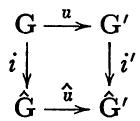
\includegraphics[keepaspectratio]{images/part001_945be03d.jpg}}

(in which \(i\) , \(i'\) are the canonical injections) is commutative. If \(v\) is a continuous homomorphism of \(\mathbf{G}'\) into a Hausdorff abelian topological group \(\mathbf{G}''\) , and if \(w = v \circ u\) , then it is follows immediately that \(\hat{w} = \hat{v} \circ \hat{u}\) .

Let H be a closed subgroup of G and let E = G/H. Let \(j: H \to G\) and \(p: G \to E\) be the canonical mappings. Let \(\overline{H}\) be the closure of H in \(\hat{G}\) ; \(\overline{H}\) is a complete group and we identify it with the completion \(\hat{H}\) of H. The continuous extension \(\hat{j}\) of j to \(\hat{H}\) is evidently the canonical injection of \(\hat{H}\) in \(\hat{G}\) .

Suppose from now on that G is metrizable. Then the canonical mapping of E = G/H into \(\hat{G}/\hat{H}\) is a topological isomorphism of E onto a dense subgroup of the complete group \(\hat{G}/\hat{H}\) (Corollary 1), and thus we may identify \(\hat{G}/\hat{H}\) with \(\hat{E}\) and the continuous extension \(\hat{p}\) of p to \(\hat{G}\) with the canonical mapping of \(\hat{G}\) onto \(\hat{G}/\hat{H}\) .

COROLLARY 2. Let G, G' be two metrizable abelian topological groups; let u: G → G' be a strict morphism with kernel N and image P. Then \(\hat{u} : \hat{G} \rightarrow \hat{G}'\) is a strict morphism with kernel \(\hat{N}\) and image \(\hat{P}\) .

Let \(u = j \circ v \circ p\) be the canonical factorization of \(u\) , where \(v\) is an isomorphism of the topological group \(G/N\) onto the topological group \(u(G) = P\) . We have \(\hat{u} = \hat{j} \circ \hat{v} \circ \hat{p}\) , and we have seen that \(\hat{p}\) is the canonical mapping of \(\hat{G}\) onto \(\hat{G}/\hat{N}\) , and that \(\hat{j}\) is the canonical mapping of \(\hat{P}\) into \(\hat{G}'\) . On the other hand, \(\hat{v}\) is an isomorphism of \(\hat{G}/\hat{N}\) onto \(\hat{P}\) (Chapter III, § 3, no. 4, Proposition 5), whence the result.

COROLLARY 3. Let \(\mathbf{G}, \mathbf{G}'\) , \(\mathbf{G}''\) be three metrizable abelian topological groups and let \(u: \mathbf{G} \to \mathbf{G}'\) and \(v: \mathbf{G}' \to \mathbf{G}''\) be two strict morphisms such that the sequence \(\mathbf{G} \xrightarrow{u} \mathbf{G}' \xrightarrow{v} \mathbf{G}''\) is exact {[}i.e., \(u(\mathbf{G}) = \overline{v}^{1}(\mathbf{o})\) {]}. Then the sequence \(\hat{\mathbf{G}} \xrightarrow{\hat{u}} \hat{\mathbf{G}}' \xrightarrow{\hat{v}} \hat{\mathbf{G}}''\) is exact.

For if we put \(\mathrm{N} = u(\mathrm{G}) = \overline{v}^{1}(\mathrm{o})\) , it follows from Corollary 2 that \(\hat{N}\) is both the image of \(\hat{u}\) and the kernel of \(\hat{v}\) .

Remarks. 1) Let G be a non-Hausdorff topological group such that the Hausdorff group associated with G is metrizable; equivalently, such that the identity element of G has a countable fundamental system of neighbourhoods in G. The proof of Proposition 4 applies to this case without modification, H being an arbitrary normal subgroup of G, and shows that the Hausdorff group associated with G/H is metrizable, and that G/H is a complete group (in general not Hausdorff) whenever G is complete.

\begin{enumerate}
\def\labelenumi{\arabic{enumi})}
\setcounter{enumi}{1}
\tightlist
\item
  Let \(d\) be a left-invariant metric which defines the topology of a metrizable group G, and let H be a closed normal subgroup of G. If \(\dot{x}\) and \(\dot{y}\) are any two points of G/H, consider the distance \(d(\dot{x},\dot{y})\) of the two closed subsets \(\dot{x},\dot{y}\) in G (§ 2, no. 2); we shall see that this function is a left-invariant metric on G/H and defines the topology of this quotient group.
\end{enumerate}

Notice first that if \(x \in \dot{x}\) and \(y \in \dot{y}\) we have \(d(\dot{x}, \dot{y}) = d(x, \mathrm{H}y)\) ; for \(d(x, \mathrm{H}y) = \inf_{h \in \mathbf{H}} d(x, h y)\) , and therefore \(d(h' x, \mathrm{H} y) = d(x, \mathrm{H} y)\) for all \(h' \in \mathrm{H}\) , since \(d\) is left-invariant; this proves the assertion (§ 2, no. 2). Hence for each \(\dot{z} \in \mathrm{G} / \mathrm{H}\) we have {[}§ 2, no. 2, formula (2){]}

\[
\left| d (\dot {x}, \dot {z}) - d (\dot {y}, \dot {z}) \right| = \left| d (x, \dot {z}) - d (y, \dot {z}) \right| \leqslant d (x, y);
\]

and since this inequality is valid for all \(x \in \dot{x}\) and all \(y \in \dot{y}\) , we have \(|d(\dot{x}, \dot{z}) - d(\dot{y}, \dot{z})| \leqslant d(\dot{x}, \dot{y})\) , which shows that \(d(\dot{x}, \dot{y})\) is a metric on G/H. Moreover, for any \(z \in \dot{z}\) , we have

\[
d (\dot {z} \dot {x}, \dot {z} \dot {y}) = \inf _ {h \in \mathbf {H}} d (z x, h z y)
\]

from above; but since \(hzy = z(z^{-1}hz)y\) and since \(z^{-1}hz\) runs through H as \(h\) runs through H (H being normal), the left-invariance of \(d(x,y)\) shows that we have \(d(zx, \mathrm{Hz}) = d(x, \mathrm{Hy}) = d(\dot{x}, \dot{y})\) . Finally, if V is a neighbourhood of \(e\) in G defined by \(d(e, x) < \alpha\) , the image V of V in G/H is the set defined by \(d(\dot{e}, \dot{x}) < \alpha\) ; this completes the proof.

\subsection{VALUED DIVISION RINGS}

DEFINITION 2. An absolute value on a division ring K is a mapping \(x \to |x|\) of K into \(\mathbf{R}_{+}\) which satisfies the following conditions:

\((\mathbf{VM}_{\mathbf{I}})\) \(|x| = 0\) if and only if \(x = 0\) .

\((\mathbf{VM}_{\mathbf{II}})\quad |xy| = |x|.|y|\) for all \(x,y\) in \(\mathbf{K}\) .

\((\mathbf{VM}_{\mathbf{III}})\quad |x + y|\leqslant |x| + |y|\) for all \(x,y\) in \(\mathbf{K}\) .

By \((\mathbf{VM}_{\mathbf{II}})\) we have \(|x| = |\mathrm{I}|.|x|\) , and since by \((\mathbf{VM}_{\mathbf{I}})\) there is at least one \(x\) such that \(|x| \neq 0\) , we have \(|\mathrm{I}| = \mathrm{I}\) ; it follows that \(\mathrm{I} = |- \mathrm{I}|^2\) , hence \(|- \mathrm{I}| = \mathrm{I}\) and consequently

\[
| - x | = | - \mathrm{I} | | x | = | x |;
\]

therefore \(|x - y| \leqslant |x| + |y|\) for all \(x, y\) in \(\mathbf{K}\) . We can therefore say that \(d(x, y) = |x - y|\) is an invariant metric on the additive group \(\mathbf{K}\) , and that the mapping \(x \to |x|\) is a homomorphism of the multiplicative group \(K^{*}\) of non-zero elements of K into the multiplicative group \(R_{+}^{*}\) of real numbers \textgreater0.

The invariant metric \(|x - y|\) defines a metric space topology on K, compatible with its additive group structure (no. 1, Proposition 3); but, moreover, this topology is compatible with the division ring structure of K. For the continuity of xy on \(K \times K\) follows from the relation

\[
x y - x _ {0} y _ {0} = (x - x _ {0}) (y - y _ {0}) + (x - x _ {0}) y _ {0} + x _ {0} (y - y _ {0}),
\]

which gives

\[
\left| x y - x _ {0} y _ {0} \right| \leqslant \left| x - x _ {0} \right|. \left| y - y _ {0} \right| + \left| x _ {0} \right|. \left| y - y _ {0} \right| + \left| y _ {0} \right|. \left| x - x _ {0} \right|.
\]

Likewise, the continuity of \(x^{-1}\) at every point \(x_{0} \neq 0\) follows from the identity \(x^{-1} - x_{0}^{-1} = x^{-1} (x_{0} - x)x_{0}^{-1}\) , which gives, by \((\mathrm{VM}_{\mathrm{II}})\) ,

\[
\left| x ^ {- 1} - x _ {0} ^ {- 1} \right| = \frac {\left| x - x _ {0} \right|}{\left| x _ {0} \right| . \left| x \right|};
\]

now if \(\varepsilon > 0\) is such that \(\varepsilon < |x_0|\) , the relation \(|x - x_0| \leqslant \varepsilon\) implies \(|x| \geqslant |x_0| - \varepsilon\) , whence \(|x^{-1} - x_{0}^{-1}| \leqslant \varepsilon / |x_0| (|x_0| - \varepsilon)\) ; and this establishes the continuity of \(x^{-1}\) at the point \(x_0\) .

DEFINITION 3. A valued division ring is a division ring K endowed with the structure defined by a given absolute value on K.

A valued division ring will always be considered as endowed with the topology defined by its absolute value, which makes it a topological division ring. If \(K_{0}\) is a division subring of a valued division ring K, the restriction to \(K_{0}\) of the absolute value on K is an absolute value on \(K_{0}\) , which defines on \(K_{0}\) the topology induced by the topology of K.

Examples. 1) Let K be an arbitrary division ring. For each \(x \in \mathbf{K}\) , put \(|x| = \mathbf{i}\) if \(x \neq 0\) , and \(|0| = 0\) . The mapping \(x \to |x|\) so defined is an absolute value on K, called the improper absolute value. The topology defined by an absolute value \(|x|\) on a division ring K is discrete if and only if \(|x|\) is the improper absolute value. This condition is clearly sufficient; conversely, if the topology of K is discrete, \(|x|\) can take no value \(\alpha > 0\) other than \(\mathbf{i}\) ; for if we had \(|x_0| = \alpha < \mathbf{i}\) , the sequence \((x_0^n)\) would consist of non-zero terms and would converge to \(\mathbf{o}\) ; to deal with the case \(\alpha > \mathbf{i}\) , consider \(x_0^{-1}\) in place of \(x_0\) .

\begin{enumerate}
\def\labelenumi{\arabic{enumi})}
\setcounter{enumi}{1}
\item
  The absolute value of a real number (Chapter IV, § 1, no. 6) satisfies axioms \((\mathrm{VM}_{\mathrm{I}})\) , \((\mathrm{VM}_{\mathrm{II}})\) and \((\mathrm{VM}_{\mathrm{III}})\) , and the topology it defines on the field \(\mathbf{R}\) is the topology of the real line. On the field \(\mathbf{C}\) of complex numbers (identified with \(\mathbf{R}^2\) ) {[}resp. the division ring \(\mathbf{H}\) of quaternions (identified with \(\mathbf{R}^4\) ){]} the Euclidean norm is again an absolute value and defines the topology of the field C (resp. the division ring H) (Chapter VIII, § 1, nos. 2 and 4).
\item
  On a division ring K, a real valuation is a function v defined on \(K^{*}\) with values in R which satisfies the following conditions: a) if \(x \in K^{*}\) and \(y \in K^{*}\) , then \(v(xy) = v(x) + v(y)\) ; b) if in addition \(x + y \neq 0\) , then \(v(x + y) \geqslant \inf(v(x), v(y))\) . If a is any real number \textgreater1, we can then define an absolute value on K by putting \(|x| = a^{-v(x)}\) for \(x \neq 0\) , and \(|0| = 0\) . For the relation \(v(xy) = v(x) + v(y)\) for \(x \neq 0\) and \(y \neq 0\) implies the relation \(|xy| = |x|.|y|\) for these values of x and y, and this relation is trivially true if one of x, y is zero; likewise, from the relation \(v(x + y) \geqslant \inf(v(x), v(y))\) for \(x \neq 0\) , \(y \neq 0\) and \(x + y \neq 0\) we deduce \(|x + y| \leqslant \sup(|x|, |y|) \leqslant |x| + |y|\) , and these inequalities are still satisfied if one of x, y, \(x + y\) is zero. In particular, if \(v_{p}(x)\) is the p-adic valuation on the field Q of rational numbers (the exponent of p in the decomposition of x into a product of prime factors), then the corresponding absolute value \(|x|_{p} = p^{-v_{p}(x)}\) is called the p-adic absolute value on the field Q (cf.~Chapter III, §6, Exercise 23).
\end{enumerate}

Remark. If \(x\) is a root of unity in a valued division ring, then \(|x| = 1\) , for \(x^n = 1\) implies \(|x|^n = 1\) and hence \(|x| = 1\) . In particular, the only absolute value on a finite field is the improper absolute value, since every element \(\neq 0\) of such a field is a root of unity.

DEFINITION 4. Two absolute values on a division ring K are said to be equivalent if they define the same topology on K.

PROPOSITION 5. Two absolute values \(|x|_1, |x|_2\) on a division ring \(K\) , neither of which is the improper absolute value, are equivalent if and only if the relation \(|x|_1 < i\) implies \(|x|_2 < i\) . There exists then a real number \(\rho > 0\) such that \(|x|_2 = |x|_1^p\) for all \(x \in K\) .

The condition is necessary, for the set of all \(x \in \mathbf{K}\) such that \(|x|_1 < 1\) is the same as the set of all \(x\) such that, with respect to the topology defined by the absolute value \(|x|_1\) , \(\lim x^n = 0\) .

Suppose conversely that \(|x|_1 < \mathrm{i} \Longrightarrow |x|_2 < \mathrm{i}\) . Then \(|x|_1 > \mathrm{i} \Longrightarrow |x|_2 > \mathrm{i}\) , because \(|x^{-1}|_1 < \mathrm{i}\) and therefore \(|x^{-1}|_2 < \mathrm{i}\) . Since by hypothesis the absolute value \(|x|_1\) is not improper, there exists \(x_0 \in \mathbf{K}\) such that \(|x_0|_1 > \mathrm{i}\) . Let \(a = |x_0|_1\) , \(b = |x_0|_2\) and let \(\rho = \log b / \log a > 0\) . Let \(x \in \mathbf{K}^*\) and put \(|x|_1 = |x_0|^{\gamma}\) . If \(m\) and \(n\) are integers such that \(n > 0\) and \(m/n > \gamma\) , then \(|x|_1 < |x_0|_1^{m/n}\) , and therefore \(|x^n x_0^{-m}|_1 < \mathrm{i}\) ; hence \(|x^n x_0^{-m}|_2 < \mathrm{i}\) , \(|x|_2 < |x_0|_2^{m/n}\) . Similarly, if \(m/n < \gamma\) , we see that \(|x|_2 > |x_0|_2^{m/n}\) ; it follows therefore that \(|x|_2 = |x_0|_2^\gamma\) ; in other words

\[
\log | x | _ {2} = \gamma \log b = \gamma \rho \log a = \rho \log | x | _ {1},
\]

i.e., \(|x|_2 = |x|_1^p\) . It is now clear that the neighbourhoods of zero for the topologies defined on \(\mathbf{K}\) by \(|x|_1\) and \(|x|_2\) are identical.

Conversely, if \(|x|\) is any absolute value on \(K\) , the function \(|x|^{\circ}\) is an absolute value on \(K\) (equivalent to \(|x|\) ) for all \(\rho\) such that \(0 < \rho \leqslant 1\) . We have only to verify the inequality \(|x + y|^{\circ} \leqslant |x|^{\circ} + |y|^{\circ}\) ; and since \(|x + y|^{\circ} \leqslant (|x| + |y|)^{\circ}\) it is enough to show that, if \(a > 0\) and \(b > 0\) , we have \((a + b)^{\circ} \leqslant a^{\circ} + b^{\circ}\) for any \(\rho\) such that \(0 < \rho \leqslant 1\) . If we put \(c = a / (a + b)\) and \(d = b / (a + b)\) , we have \(c + d = 1\) , and the inequality to be proved is \(c^{\circ} + d^{\circ} \geqslant 1\) ; but this follows immediately from the relations \(c^{\circ} \geqslant c\) and \(d^{\circ} \geqslant d\) , which are valid since \(0 < c \leqslant 1\) , \(0 < d \leqslant 1\) , \(0 < \rho \leqslant 1\) .

Hence the set of values of r \textgreater{} 0 such that \(|x|^{r}\) is an absolute value is a finite or infinite interval of R with left-hand end-point o; if it is finite, it is evidently closed; for if we have \(|x + y|^{r} \leqslant |x|^{r} + |y|^{r}\) for any x, y in K and all r such that \(0 < r < r_{0}\) , then by continuity the inequality is still valid for \(r = r_{0}\) . If \(|x|^{r}\) is an absolute value for all r \textgreater{} 0, then we have

\[
| x + y | \leqslant (| x | ^ {r} + | y | ^ {r}) ^ {1 / r}
\]

for all \(x\) and \(y\) in \(\mathbf{K}\) and all \(r > 0\) . Now, if \(a, b\) are two real numbers \(\geqslant 0\) , we have \(\lim_{r \to \infty} (a^r + b^r)^{1/c} = \sup (a, b)\) ; for, supposing for example that \(a \geqslant b\) , we have \(a \leqslant (a^r + b^r)^{1/r} \leqslant 2^{1/r} a\) , and the result follows by letting \(r \to +\infty\) .

Thus, if \(|x|^r\) is an absolute value for all \(r > 0\) , we have

\[
| x + y | \leqslant \sup (| x |, | y |)
\]

which can be expressed by saying that \(v(x) = -\log |x| (x \neq 0)\) is a valuation on K.

Remark. The proof of Proposition 5 shows that, if the topology defined by \(|x|_2\) is coarser than that defined by \(|x|_1\) , and if \(|x|_1\) is not improper, then \(|x|_1\) and \(|x|_2\) are equivalent, for the relation \(|x|_2 < 1\) then implies \(|x|_2 < 1\) . Thus the topologies defined by two absolute values on \(K\) , neither of which is improper, cannot be comparable without being identical.

PROPOSITION 6. The completion \(\hat{\mathbf{K}}\) of a division ring \(\mathbf{K}\) endowed with an absolute value \(|x|\) is a division ring, and the function \(|x|\) can be extended by continuity to an absolute value on \(\hat{\mathbf{K}}\) , which defines the topology of \(\hat{\mathbf{K}}\) .

Let \(\mathfrak{F}\) be a Cauchy filter on K (with respect to the additive uniformity) which does not have o as a cluster point; to show that \(\hat{\mathbf{K}}\) is a division ring it is enough to establish that the image of \(\mathfrak{F}\) under the mapping \(x \to x^{-1}\) is a Cauchy filter base (Chapter III, § 6, no. 8, Proposition 7). Now, by hypothesis there exists a real number \(\alpha > 0\) and a set \(\mathrm{A} \in \mathfrak{F}\) such that \(|x| \geqslant \alpha\) for all \(x \in \mathrm{A}\) ; on the other hand, for each \(\varepsilon > 0\) there exists a set \(\mathrm{B} \in \mathfrak{F}\) such that \(\mathrm{B} \subset \mathrm{A}\) and \(|x - y| \leqslant \varepsilon\) for all \(x \in \mathrm{B}\)

and \(y\in \mathbf{B}\) ; hence

\[
\left| x ^ {- 1} - y ^ {- 1} \right| = \frac {\left| x - y \right|}{\left| x \right| . \left| y \right|} \leqslant \frac {\varepsilon}{\alpha^ {2}},
\]

and the first part of the proposition follows. The invariant metric \(|x - y| = d(x, y)\) extends by continuity to a metric on \(\hat{\mathbf{K}}\) (§ 2, no. 1, Proposition 1) which defines the topology of \(\hat{\mathbf{K}}\) and is invariant by the principle of extension of identities; we continue to denote this invariant metric by \(d(x, y)\) . If we put \(|x| = d(0, x)\) for \(x \in \hat{\mathbf{K}}\) , it is clear that \(|x|\) is the extension by continuity of the function \(|x|\) on \(\mathbf{K}\) and is therefore an absolute value on \(\hat{\mathbf{K}}\) by the principle of extension of identities.

\subsection{NORMED SPACES OVER A VALUED DIVISION RING}

DEFINITION 5. If E is a (left) vector space over a non-discrete valued division ring K, a norm on E is a mapping \(\mathbf{x} \to p(\mathbf{x})\) of E into \(\mathbf{R}_+\) which satisfies the following axioms:

\[
\left(\mathrm{NO} _ {\mathbf {I I}}\right) \quad p (\boldsymbol {x} + \boldsymbol {y}) \leqslant p (\boldsymbol {x}) + p (\boldsymbol {y}) \text {   for   all   } \boldsymbol {x}, \boldsymbol {y} \text {   in   } \mathbf {E};
\]

\[
\left(\mathrm{NO} _ {\mathbf {I I I}}\right) \quad p (t \boldsymbol {x}) = | t | p (\boldsymbol {x}) \text {for all} t \in \mathrm{K} \text {and all} \boldsymbol {x} \in \mathrm{E}.
\]

The normed spaces most frequently met with have either R or C as field of scalars (with the usual absolute value).

From \((\mathrm{NO}_{\mathrm{III}})\) it follows in particular that \(p(-x)=p(x)\) ; hence if we put \(d(x,y)=p(x-y)\) , d is an invariant metric on the additive group E, and defines a metric space topology compatible with the additive group structure of E (no. 1, Proposition 3); moreover, the mapping

\[
(t, \boldsymbol {x}) \rightarrow t \boldsymbol {x}
\]

is continuous on \(\mathbf{K} \times \mathbf{E}\) ; for we have

\[
t \boldsymbol {x} - t _ {0} \boldsymbol {x} _ {0} = (t - t _ {0}) (\boldsymbol {x} - \boldsymbol {x} _ {0}) + (t - t _ {0}) \boldsymbol {x} + t _ {0} (\boldsymbol {x} - \boldsymbol {x} _ {0})
\]

and therefore

\[
p (t \boldsymbol {x} - t _ {0} \boldsymbol {x} _ {0}) \leqslant | t - t _ {0} | p (\boldsymbol {x} - \boldsymbol {x} _ {0}) + | t - t _ {0} | p (\boldsymbol {x}) + | t _ {0} | p (\boldsymbol {x} - \boldsymbol {x} _ {0}),
\]

which shows that the left-hand side can be made as small as we please by taking \(|t - t_{0}|\) and \(p(x - x_{0})\) sufficiently small.

DEFINITION 6. If K is a non-discrete valued division ring, a vector space E over K, endowed with the structure defined by a given norm on E, is called a normed space over K.

A normed space will always be considered as endowed with the topology and the uniformity defined by its norm.

Examples. 1) On a non-discrete valued division ring K, considered as a (left or right) vector space over itself, the absolute value \(|x|\) is a norm.

\begin{enumerate}
\def\labelenumi{\arabic{enumi})}
\setcounter{enumi}{1}
\item
  The expression \(||x|| = \sqrt{\sum_{i=1}^{n} x_i^2}\) , which we have called the Euclidean norm on the space \(\mathbf{R}^n\) (Chapter VI, § 2) is evidently a norm in the sense of Definition 5. So are the functions \(\sup_{1 \leqslant i \leqslant n} |x_i|\) and \(\sum_{i=1}^{n} |x_i|\) .
\item
  Let \(\mathcal{B}(\mathrm{E};\mathrm{K})\) be the set of all functions \(f\) on a set \(\mathrm{E}\) which take their values in a non-discrete valued division ring \(\mathbf{K}\) and are such that the real-valued function \(x\to |f(x)|\) is bounded on \(\mathbf{E}\) . This set is clearly a vector subspace of the (left or right) vector space \(\mathbf{K}^{\mathbf{E}}\) of all mappings of \(\mathbf{E}\) into \(\mathbf{K}\) . If we put \(p(f)=\sup_{x\in\mathbb{E}}|f(x)|\) , then \(p\) is a norm on the vector space \(\mathcal{B}(\mathrm{E};\mathrm{K})\) (cf.~Chapter X, § 1).
\end{enumerate}

* 4) On the vector space \(\mathcal{C}(\mathrm{I};\mathbf{R})\) of all finite continuous real-valued functions defined on the interval \(\mathbf{I} = [0,1]\) of \(\mathbf{R}\) , the function

\[
p (x) = \int_ {0} ^ {1} | x (t) | d t
\]

is a norm. *

In a normed space E, the (closed) ball B with centre o and radius i, that is to say the set of all \(x \in E\) such that \(p(x) \leqslant i\) , will be called the unit ball in E. Let us show that a fundamental system of neighbourhoods of o in E is formed by the transforms of the unit ball by the homotheties \(x \to tx\) , where t runs through the set of non-zero elements of K. The image of B under this homothety is the closed ball with centre o and radius \(|t|\) ; hence it is enough to show that for each real number r \textgreater{} o there exists \(t \in K\) such that \(o < |t| < r\) . Now since the absolute value of K is not improper, there exists \(t_{0} \in K\) such that \(o < |t_{0}| < i\) ; it is therefore enough to take \(t = t_{0}^{n}\) , where n is a sufficiently large integer, in order that \(|t| = |t_{0}|^{n} < r\) .

DEFINITION 7. Two norms on a vector space E (over a non-discrete valued division ring K) are said to be equivalent if they define the same topology on E.

PROPOSITION 7. Two norms \(p, q\) on a vector space \(E\) are equivalent if and only if there exist two numbers \(a > 0, b > 0\) such that

\[
a. p (\pmb {x}) \leqslant q (\pmb {x}) \leqslant b. p (\pmb {x})\tag{I}
\]

for all \(x \in E\) .

These inequalities are sufficient, for it follows from the relation \(a.p(x) \leqslant q(x)\) that, for each \(r > 0\) , the closed ball with centre \(o\) and radius \(ar\) (relative to the norm \(q\) ) is contained in the closed ball with centre \(o\) and radius \(r\) (relative to the norm \(p\) ); hence the topology defined by \(q\) is finer than the topology defined by \(p\) . Similarly the inequality \(q(x) \leqslant b.p(x)\) shows that the topology defined by \(p\) is finer than that defined by \(q\) , and hence \(p\) and \(q\) are equivalent.

Let us now show that the inequalities (1) are necessary. If the topology defined by \(q\) is finer than the topology defined by \(p\) , then the unit ball with respect to \(p\) contains a closed ball with centre \(o\) and radius \(\alpha > 0\) with respect to \(q\) ; i.e., the relation \(q(x) \leqslant \alpha\) implies \(p(x) \leqslant 1\) . If \(t_0 \in K\) is such that \(0 < |t_0| < 1\) , then for each \(x \neq 0\) in \(E\) there is a unique rational integer \(k\) such that \(\alpha |t_0| < q(t_0^k x) \leqslant \alpha\) ; therefore \(p(t_0^k x) \leqslant 1\) , so that

\[
p (\boldsymbol {x}) \leqslant \frac {\mathrm{I}}{\left| t _ {0} \right| ^ {k}} \leqslant \frac {\mathrm{I}}{\alpha \left| t _ {0} \right|} q (\boldsymbol {x});
\]

putting \(a = \alpha |t_0|\) we have therefore \(a.p(x) \leqslant q(x)\) for all \(x \neq 0\) , and this inequality is also valid when \(x = 0\) . Similarly we show that if the topology defined by \(p\) is finer than that defined by \(q\) , there exists \(b > 0\) such that \(q(x) \leqslant b.p(x)\) .

Example. In the space \(R^{n}\) , the three norms

\[
\sqrt {\sum_ {i = 1} ^ {n} x _ {i} ^ {2}}, \quad \sup _ {1 \leqslant i \leqslant n} | x _ {i} | \quad \text { and } \quad \sum_ {i = 1} ^ {n} | x _ {i} |
\]

are equivalent, because we have

\[
\sup _ {1 \leqslant i \leqslant n} | x _ {i} | \leqslant \sqrt {\sum_ {i = 1} ^ {n} x _ {i} ^ {2}} \leqslant \sum_ {i = 1} ^ {n} | x | _ {i} \leqslant n. \sup _ {1 \leqslant i \leqslant n} | x _ {i} |.\tag{2}
\]

PROPOSITION 8. Let E be a normed space over a non-discrete valued division ring, let p be the norm on E, and let \(\hat{E}\) be the additive topological group which is the completion of the additive group E. Then the function \((t, x) \to tx\) can be extended by continuity to \(\hat{K} \times \hat{E}\) and defines on \(\hat{E}\) a vector space structure over \(\hat{K}\) ; the norm p can be extended by continuity to a norm \(\overline{p}\) on \(\hat{E}\) which defines the topology of \(\hat{E}\) .

The extension of tx by continuity is a particular case of the theorem of extension of a continuous bilinear mapping of a product of two abelian groups into a third (Chapter III, § 6, no. 5, Theorem 1); we have \(\mathbf{I} \cdot \mathbf{x} = \mathbf{x}\) and \(t(ux) = (tu)x\) for \(t \in \hat{\mathbf{K}}\) , \(u \in \hat{\mathbf{K}}\) and \(\mathbf{x} \in \hat{\mathbf{E}}\) , by the principle of extension of identities; hence the external law \((t, \mathbf{x}) \to tx\) indeed defines on \(\hat{\mathbf{E}}\) a structure of a vector space over \(\hat{\mathbf{K}}\) . On the other hand, the invariant metric \(\overline{d}(\mathbf{x}, \mathbf{y}) = \overline{p}(\mathbf{x} - \mathbf{y})\) extends to an invariant metric \(\overline{d}\) on \(\hat{\mathbf{E}}\) ( \(\S 2\) , no. 1, Proposition 1) which defines the topology of \(\hat{\mathbf{E}}\) ; if we set \(\overline{p}(\mathbf{x}) = \overline{d}(\mathrm{o}, \mathbf{x})\) , then \(\overline{p}\) is the extension of \(p\) by continuity, and satisfies axioms \((\mathrm{NO}_{\mathbf{I}})\) and \((\mathrm{NO}_{\mathbf{II}})\) ; by virtue of the continuity of \(tx\) on \(\hat{\mathbf{K}} \times \hat{\mathbf{E}}\) , \(\overline{p}\) also satisfies \((\mathrm{NO}_{\mathbf{III}})\) (principle of extension of identities) and is therefore a norm on \(\hat{\mathbf{E}}\) .

When we have to consider a definite normed space structure on a vector space E, we shall usually denote the norm of a vector x by \(\|x\|\) , unless this notation is likely to lead to confusion.

\subsection{QUOTIENT SPACES AND PRODUCT SPACES OF NORMED SPACES}

PROPOSITION 9. Let E be a normed space over a non-discrete valued division ring K, and let H be a closed vector subspace of E. If, for each class \(\dot{\mathbf{x}}\in\mathbf{E}/\mathbf{H}\) , we put \(||\dot{\mathbf{x}}||=\inf_{\mathbf{x}\in\dot{\mathbf{x}}}\|\mathbf{x}||\) , the function \(||\dot{\mathbf{x}}||\) is a norm on the vector space E/H,

and the topology defined by this norm is the quotient by H of the topology of E. By Remark 2 of no. 1, \(d(\dot{\boldsymbol{x}}, \dot{\boldsymbol{y}}) = ||\dot{\boldsymbol{x}} - \dot{\boldsymbol{y}}||\) is an invariant metric on E/H which defines the quotient by H of the topology of E. It remains only to show that \(||t\dot{\boldsymbol{x}}|| = |t|.||\dot{\boldsymbol{x}}||\) , and this follows immediately from the definition of \(||\dot{\boldsymbol{x}}||\) {[}Chapter IV, § 5, no. 7, formula (23){]}.

The norm \(||\dot{\pmb{x}}||\) may also be interpreted as follows: it is the distance (in E) of every point \(\pmb{x} \in \dot{\pmb{x}}\) from the subspace H, for the points of \(\dot{\pmb{x}}\) are the points \(\pmb{x} - \pmb{z}\) , where \(\pmb{z}\) runs through H.

PROPOSITION 10. Let \((\mathbf{E}_i)_{1 \leqslant i \leqslant n}\) be a finite family of normed spaces over a non-discrete valued division ring K, and let \(\mathbf{E} = \prod_{i=1}^{n} \mathbf{E}_i\) be the product vector space. If for each \(x = (x_i) \in \mathbf{E}\) we put \(||x|| = \sup_{1 \leqslant i \leqslant n} ||x_i||\) , then the function \(||x||\) is a norm on E, and the topology it defines on E is the product of the topologies of the \(\mathbf{E}_i\) .

For if \(\pmb{x} = (\pmb{x}_i)\) and \(\pmb{y} = (\pmb{y}_i)\) , we have \(\pmb{x} + \pmb{y} = (\pmb{x}_i + \pmb{y}_i)\) and therefore

\[
\begin{array}{r l} | | \boldsymbol {x} + \boldsymbol {y} | | = & \sup _ {i} | | \boldsymbol {x} _ {i} + \boldsymbol {y} _ {i} | | \leqslant \sup _ {i} (| | \boldsymbol {x} _ {i} | | + | | \boldsymbol {y} _ {i} | |) \\ & \leqslant \sup _ {i} | | \boldsymbol {x} _ {i} | | + \sup _ {i} | | \boldsymbol {y} _ {i} | | = | | \boldsymbol {x} | | + | | \boldsymbol {y} | |. \end{array}
\]

On the other hand, it is clear that \(||tx|| = |t|.||x||\) , and that if \(||x|| = 0\) , then \(||x_i|| = 0\) and therefore \(x_i = 0\) for \(1 \leqslant i \leqslant n\) , so that \(x = 0\) ; hence \(||x||\) is a norm on E. Also the relation \(||x|| < a\) is equivalent to the \(n\) relations \(||x_i|| < a\) , and therefore the norm \(||x||\) defines the product topology on E.

Similarly we can show that the functions \(\sum_{i=1}^{n} \|x_i\|\) and \(\sqrt{\sum_{i=1}^{n} \|x_i\|^2}\) are norms on E; the inequalities (2) show that all three norms are equivalent.

In particular, in the (left or right) vector space \(K^{n}\) , if we put

\[
p _ {1} (\boldsymbol {x}) = \sup _ {i} | x _ {i} |, \quad p _ {2} (\boldsymbol {x}) = \sum_ {i = 1} ^ {i = 1} | x _ {i} |, \quad p _ {3} (\boldsymbol {x}) = \sqrt {\sum_ {i = 1} ^ {n} | x _ {i} | ^ {2}}
\]

for \(\pmb{x} = (x_{i})_{1\leqslant i\leqslant n}\) , then the three functions \(p_1, p_2, p_3\) are equivalent norms which define on \(\mathbf{K}^n\) the topology which is the product of the topologies of the factors \(\mathbf{K}\) .

\subsection{CONTINUOUS MULTILINEAR FUNCTIONS}

THEOREM 1. Let \(\mathbf{E}_i(\mathbf{i} \leqslant i \leqslant n)\) and \(\mathbf{F}\) be normed spaces over a non-discrete valued division ring \(\mathbf{K}\) , and let \(f\) be a multilinear mapping of \(\prod_{i=1}^{n} \mathbf{E}_i\) into \(\mathbf{F}\) . Then \(f\) is continuous on \(\prod_{i=1}^{n} \mathbf{E}_i\) if and only if there exists a real number \(a > 0\) such that, for all \(\boldsymbol{x}_i \in \mathbf{E}_i\) ( \(\mathbf{i} \leqslant i \leqslant n\) ), we have

\[
\left| \left| f \left(\boldsymbol {x} _ {1}, \boldsymbol {x} _ {2}, \dots , \boldsymbol {x} _ {n}\right) \right| \right| \leqslant a. \left| \left| \boldsymbol {x} _ {1} \right| \right|. \left| \left| \boldsymbol {x} _ {2} \right| \right|. \dots . \left| \left| \boldsymbol {x} _ {n} \right| \right|.\tag{3}
\]

The condition is necessary. For if \(f\) is continuous at the point \((\mathbf{o}, \mathbf{o}, \ldots, \mathbf{o})\) there exists a number \(b > 0\) such that the relations \(||\boldsymbol{x}_i|| \leqslant b\) ( \(\mathbf{i} \leqslant i \leqslant n\) ) imply \(||f(\boldsymbol{x}_1, \ldots, \boldsymbol{x}_n)|| \leqslant \mathbf{i}\) . Let \(t_0\) be an element of \(\mathbf{K}\) such that \(0 < |t_0| < \mathbf{i}\) ; then for every point \((\boldsymbol{x}_i) \in \prod_{i=1}^{n} \mathrm{E}_i\) such that none of the \(\boldsymbol{x}_i\) is zero, there exist \(n\) rational integers \(k_i\) such that \(b|t_0| < ||t_0^k |\boldsymbol{x}_i|| \leqslant b\) ; consequently we have

\[
\left| t _ {0} \right| ^ {k _ {1} + k _ {2} + \dots + k _ {n}} \left| \left| f \left(\boldsymbol {x} _ {1}, \boldsymbol {x} _ {2}, \dots , \boldsymbol {x} _ {n}\right) \right| \right| \leqslant 1;
\]

on the other hand we have \(\frac{\mathbf{I}}{|t_0|^k_i} \leqslant \frac{\mathbf{I}}{b|t_0|} ||\boldsymbol{x}_i||\) , and the relation (3) therefore follows, with \(a = (\mathbf{I}/b|t_0|)^n\) . This relation is evidently still valid when one of the \(\boldsymbol{x}_i\) is zero.

The condition is sufficient. We shall show that, if it is satisfied, \(f\) is continuous at every point \((\pmb{a}_i)\) of \(\prod_{i=1}^{n} \mathbf{E}_i\) . We can write

\[
f \left(x _ {1}, \dots , x _ {n}\right) - f \left(a _ {1}, \dots , a _ {n}\right) = \sum_ {i = 1} ^ {n} f \left(a _ {1}, \dots , a _ {i - 1}, x _ {i} - a _ {i}, x _ {i + 1}, \dots , x _ {n}\right).
\]

Now, using (3), the conditions \(||\pmb{x}_i - \pmb{a}_i|| \leqslant r\) ( \(1 \leqslant i \leqslant n\) ) imply that

\[
\left| \left| f \left(\boldsymbol {a} _ {1}, \dots , \boldsymbol {a} _ {i - 1}, \boldsymbol {x} _ {i} - \boldsymbol {a} _ {i}, \boldsymbol {x} _ {i + 1}, \dots , \boldsymbol {x} _ {n}\right) \right| \right| \leqslant a r \prod_ {k \neq i} ^ {n} \left(\left| \left| \boldsymbol {a} _ {k} \right| \right| + r\right);
\]

hence, if \(c\) is the maximum of the numbers \(\| \pmb{a}_i \| (\mathbf{i} \leqslant i \leqslant n)\) , we have

\[
\left| \left| f \left(\boldsymbol {x} _ {1}, \dots , \boldsymbol {x} _ {n}\right) - f \left(\boldsymbol {a} _ {1}, \dots , \boldsymbol {a} _ {n}\right) \right| \right| \leqslant n a r (c + r) ^ {n - 1}.
\]

Since the right-hand side of this inequality is a polynomial in r with zero constant term, it tends to o as r tends to o; hence f is continuous.

Remark. Two of the propositions proved earlier are consequences of this theorem: the continuity of the bilinear function \(tx\) , by virtue of the relation \(||tx|| = |t|.||x||\) ; and Proposition 7, by applying Theorem 1 to the identity mapping of E, considered as a linear mapping of the space E, endowed with the norm \(p\) into the space E endowed with the norm \(q\) (or vice versa).

\subsection{ABSOLUTELY SUMMABLE FAMILIES IN A NORMED SPACE}

DEFINITION 8. In a normed space E, a family \((\pmb{x}_{t})\) of points of E is said to be absolutely summable if the family \((||\pmb{x}_{t}||)\) of norms of the \(\pmb{x}_{t}\) is summable in R.

This concept appears to depend on the norm chosen on E; but by Proposition 7 of no. 3 and the comparison principle for summable families of real numbers, a family which is absolutely summable with respect to a norm p on E is absolutely summable with respect to any norm on E which is equivalent to p.

If \((\pmb{x}_t)_{i\in I}\) is a family of points of \(E\) which is summable and absolutely summable, we have

\[
\left| \left| \sum_ {i \in I} x _ {i} \right| \right| \leqslant \sum_ {i \in I} | | x _ {i} | |.\tag{4}
\]

Indeed, for each finite subset J of I we have \(\left\|\sum_{i\in J}x_{i}\right\| \leqslant \sum_{i\in J}||x_{i}||\) , and the inequality (4) follows by passing to the limit with respect to the directed set of finite subsets of I.

PROPOSITION 11. In a complete normed space E, every absolutely summable family is summable.

For if \((\pmb{x}_i)\) is an absolutely summable family in \(\mathbf{E}\) , then for each \(\varepsilon > 0\) there is a finite subset \(J\) of the index set \(I\) such that, for each finite subset \(H\) of \(I\) which does not meet \(J\) , we have \(\sum_{i \in H} ||\pmb{x}_i|| \leqslant \varepsilon\) ; hence a fortiori \(\left\| \sum_{i \in H} \pmb{x}_i \right\| \leqslant \varepsilon\) , and this proves the proposition, since \(E\) is complete (Cauchy's criterion, Chapter III, § 5, no. 2, Theorem 1).

A series whose general term is \(x_{n}\) is said to be absolutely convergent in E if the series whose general term is \(\|x_{n}\|\) is convergent in R, or (equivalently) if the family \((x_{n})\) is absolutely summable; consequently (Chapter III, § 5, no. 7, Proposition 9):

COROLLARY. In a complete normed space E, every absolutely convergent series is commutatively convergent.

The converse of Proposition 11 is in general false.

Consider for example the space \(\mathcal{B}(\mathbf{N};\mathbf{R})\) of bounded sequences \(x = (x_{n})_{n\in \mathbb{N}}\) of real numbers, with the norm \(\| x\| = \sup_n |x_n|\) . Let \(x_{m}\) be the sequence \((x_{mn})_n\in \mathbb{N}\) such that \(x_{mn} = 0\) if \(m\neq n\) and \(x_{mm} = 1 / m\) for \(m\geqslant 1\) . It is immediately verified that the sequence \((x_m)_{m\in \mathbb{N}}\) is summable in \(\mathcal{B}(\mathbf{N};\mathbf{R})\) and that its sum is the element \(y = (y_{n})\) such that \(y_0 = 0\) and \(y_{n} = 1 / n\) if \(n\geqslant 1\) ; but since \(\| x_m\| = 1 / m\) , the sequence of norms of the \(x_{m}\) is not summable in \(\mathbf{R}\) .

However, we have seen in Chapter VII, § 3, no. 1, that every summable family in \(\mathbf{R}^n\) is absolutely summable.

\subsection{NORMED ALGEBRAS OVER A VALUED FIELD}

DEFINITION 9. If A is an algebra over a non-discrete valued field K, a norm \(p(x)\) on A (A being considered as a vector space over K) is said to be compatible with the algebra structure of A if the topology it defines is compatible with the ring structure of A. An algebra over K, endowed with the structure defined by a norm compatible with the algebra structure, is called a normed algebra.

If A is a normed algebra over K, and if \(p(\boldsymbol{x})\) is the norm on A, the bilinear mapping \((\boldsymbol{x}, \boldsymbol{y}) \to \boldsymbol{x}\boldsymbol{y}\) of A × A into A is continuous, by hypothesis; hence by Theorem 1 of no. 5 there exists a real number a \textgreater{} 0 such that \(p(\boldsymbol{x}\boldsymbol{y}) \leqslant a.p(\boldsymbol{x})p(\boldsymbol{y})\) . Replacing \(p(\boldsymbol{x})\) by the equivalent norm \(a.p(\boldsymbol{x})\) , we may therefore always assume that the norm \(||\boldsymbol{x}||\) on a normed algebra A is such that

\[
\left| \left| x y \right| \right| \leqslant \left| \left| x \right| \right|. \left| \left| y \right| \right|.\tag{5}
\]

It follows from (5) by induction that, for each integer \(n > 0\) , we have

\[
\left| \left| x ^ {n} \right| \right| \leqslant \left| \left| x \right| \right| ^ {n}.\tag{6}
\]

Examples. 1) Let K be a valued division ring and let \(K'\) be a subfield of the centre of K such that the trace on \(K'\) of the absolute value \(|x|\) of K is not the improper absolute value on \(K'\) . Then K, with \(|x|\) as norm, is a normed algebra over \(K'\) .

\begin{enumerate}
\def\labelenumi{\arabic{enumi})}
\setcounter{enumi}{1}
\item
  Let K be a non-discrete valued field and let \(\mathbf{M}_{n}(\mathbf{K})\) be the ring of square matrices of order n over K. Regarded as a vector space over K, \(\mathbf{M}_{n}(\mathbf{K})\) is isomorphic to \(K^{n^{2}}\) . If for each \(X = (x_{ij}) \in \mathbf{M}_{n}(\mathbf{K})\) we define \(\|X\| = \sup_{i,j} |x_{ij}|\) , then \(\|X\|\) is a norm on \(\mathbf{M}_{n}(\mathbf{K})\) , and the topology defined by this norm is the product topology on \(K^{n^{2}}\) (Proposition 10); from this it follows (because of the continuity of polynomials in any number of variables over K) that this norm is compatible with the K-algebra structure of \(\mathbf{M}_{n}(\mathbf{K})\) .
\item
  The set \(\mathcal{B}(\mathbf{X};\mathbf{K})\) of all functions \(f\) on a set \(\mathbf{X}\) with values in a non-discrete valued field \(\mathbf{K}\) , such that \(x\to |f(x)|\) is bounded on \(\mathbf{X}\) , is an algebra over \(\mathbf{K}\) ; the norm \(\| f\| = \sup_{x\in \mathbf{X}}|f(x)|\) is compatible with the ring structure of \(\mathcal{B}(\mathbf{X};\mathbf{K})\) , because we have \(\| fg\| \leqslant \| f\| .\| g\|\) (cf.~Chapter X, § 1).
\end{enumerate}

Let \(\mathfrak{a}\) be a closed two-sided ideal in a normed algebra \(\mathbf{A}\) . If in the quotient algebra \(\mathbf{A} / \mathfrak{a}\) we put \(||\dot{\mathbf{x}}|| = \inf_{\mathbf{x}\in \dot{\mathbf{x}}}||\mathbf{x}||\) , we get a norm on \(\mathbf{A} / \mathfrak{a}\) which defines the topology which is the quotient by \(\mathfrak{a}\) of the topology of \(\mathbf{A}\) (Proposition 9); since this quotient topology is compatible with the quotient ring structure of \(\mathbf{A} / \mathfrak{a}\) (Chapter III, § 6, no. 4) it follows that the quotient algebra \(\mathbf{A} / \mathfrak{a}\) , with the norm \(||\mathbf{x}||\) , is a normed algebra.

Likewise, if \((\mathbf{A}_i)_{1 \leqslant i \leqslant n}\) is a family of \(n\) normed algebras over a valued field \(\mathbf{K}\) , and if in the product algebra \(\mathbf{A} = \prod_{i=1}^{n} \mathbf{A}_i\) we put \(||\boldsymbol{x}|| = \sup_{i} ||\boldsymbol{x}_i||\) , where \(\boldsymbol{x} = (\boldsymbol{x}_i)\) , we have a norm on \(\mathbf{A}\) which defines the product of the topologies of the \(\mathbf{A}_i\) (Proposition 10); since this topology is compatible with the ring structure of \(\mathbf{A}\) (Chapter III, § 6, no. 4), it follows that the product algebra \(\mathbf{A}\) , with the norm \(||\boldsymbol{x}||\) , is a normed algebra.

Let A be a normed algebra over a valued field K. The completion \(\hat{\mathbf{A}}\) of A (Chapter III, § 6, no. 5, Proposition 6) is also endowed with a \(\hat{\mathbf{K}}\) -vector space structure (no. 3, Proposition 8), and it is clear from the principle of extension of identities that we have \(t(xy) = (tx)y = x(ty)\) for all \(t \in \hat{\mathbf{K}}\) and all \(x, y \in \hat{\mathbf{A}}\) . Hence \(\hat{\mathbf{A}}\) is an algebra over \(\hat{\mathbf{K}}\) ; on the other hand (no. 3, Proposition 8), the norm on A extends by continuity to a norm which defines the topology of \(\hat{\mathbf{A}}\) , and therefore \(\hat{\mathbf{A}}\) , endowed with this norm, is a normed algebra over the field \(\hat{\mathbf{K}}\) .

If \((\pmb{x}_{\lambda})_{\lambda \in \mathbf{L}}\) and \((\pmb{y}_{\mu})_{\mu \in \mathbf{M}}\) are two absolutely summable families in a normed algebra \(\mathbf{A}\) , the family \((\pmb{x}_{\lambda}\pmb{y}_{\mu})_{(\lambda, \mu) \in \mathbf{L} \times \mathbf{M}}\) is absolutely summable, because \(||\pmb{x}_{\lambda}\pmb{y}_{\mu}|| \leqslant ||\pmb{x}_{\lambda}|| \cdot ||\pmb{y}_{\mu}||\) (Chapter IV, § 7, no. 3, Proposition 1); if in addition \(\mathbf{A}\) is complete, all three families are summable and we have

\[
\sum_ {(\lambda , \mu) \in \mathbf {L} \times \mathbf {M}} x _ {\lambda} y _ {\mu} = \left(\sum_ {\lambda \in \mathbf {L}} x _ {\lambda}\right) \left(\sum_ {\mu \in \mathbf {M}} y _ {\mu}\right)
\]

by the associativity of the sum on the left-hand side (Chapter III, § 5, no. 3, formula (2)).

If the normed algebra A has an identity element \(e \neq 0\) , the mapping \(t \rightarrow te\) is an isomorphism of the field structure of K onto that of the subfield Ke of A; this isomorphism is also an isomorphism of the topological field structure of K onto that of Ke (the topology of the latter being induced by that of A), for the restriction \(\|te\|\) of the norm of A to Ke is a norm equivalent to the absolute value

\[
| t | = \frac {\mathrm{I}}{| | e | |} | | t e | |.
\]

If \(||e|| = 1\) we have \(||te|| = |t|\) , and we can then identify the valued field \(K\) with the normed subfield \(Ke\) of \(A\) , and in particular we may denote the identity element of \(A\) by the symbol \(I\) .

In what follows we shall be concerned only with normed algebras which have an identity element e, and in which the norm satisfies the inequality (5); putting x = y = e in this inequality, it follows that \(\|e\| \geqslant 1\) .

PROPOSITION 12. If the series whose general term is \(z^n\) is convergent in A, then \(e - z\) is a unit of A and we have

\[
(e - z) ^ {- 1} = \sum_ {n = 0} ^ {\infty} z ^ {n}.\tag{7}
\]

Conversely, if \(||z|| < 1\) and if \(e - z\) is a unit in \(A\) , then the series whose general term is \(z^n\) is convergent and formula (7) is valid.

For each \(p > 0\) we have

\[
(e - z) \sum_ {n = 0} ^ {p} z ^ {n} = e - z ^ {p + 1}.\tag{8}
\]

If the series whose general term is \(z^{n}\) is convergent and if y is its sum, then \(z^{n}\) tends to o as \(n \to +\infty\) ; hence by passing to the limit in (8) we have \((e - z)y = e\) ; similarly we prove that \(y(e - z) = e\) , and hence \(y = (e - z)^{-1}\) (note that this part of the argument is valid in any topological ring which has an identity element).

Conversely, if \(||z|| < 1\) , then since \(||z^{p+1}|| \leqslant ||z||^{p+1}\) , it follows that \(z^{p+1}\) tends to o as \(p \to +\infty\) ; multiplying both sides (8) on the left by \((e - z)^{-1}\) and letting \(p\) tend to infinity, we see that the series whose general term is \(z^n\) converges and has \((e - z)^{-1}\) as its sum.

COROLLARY. Let A be a complete normed algebra. Then for each \(z \in \mathbf{A}\) such that \(||z|| < 1\) , \(e - z\) is a unit in A.

The series whose general term is \(z^n\) is absolutely convergent, since \(||z^n|| \leqslant ||z||^n\) for \(n > 0\) , and is therefore convergent, since \(A\) is complete (no. 6, Proposition 11).

PROPOSITION 13. Let G be the group of units of a complete normed algebra A. Then G is an open subset of A; the topology induced on G by the topology of A is compatible with the group structure of G; and G, endowed with this topology, is a complete group (with respect to each of its two uniformities).

The corollary to Proposition 12 shows that G contains a neighbourhood V of e in A; hence, for each \(x_{0} \in G\) , the elements of \(x_{0}V\) are units, and \(x_{0}V\) is a neighbourhood of \(x_{0}\) in A, since \(x \to x_{0}x\) is a homeomorphism of A onto itself ( \(x_{0}\) being a unit of A). Hence G is open in A.

To show that the topology induced on \(\mathbf{G}\) by the topology of \(\mathbf{A}\) is compatible with the group structure of \(\mathbf{G}\) , it is sufficient to show that the function \(x^{-1}\) is continuous on \(\mathbf{G}\) . Let \(x_0 \in \mathbf{G}\) , and for each \(x \in \mathbf{G}\) , write \(\boldsymbol{x}\) in the form \(x = x_0 (e + u)\) , so that \(u = x_0^{-1}(x - x_0)\) ; then \(||\boldsymbol{u}|| \leqslant ||x_0^{-1}|| \cdot ||\boldsymbol{x} - x_0||\) , and thus if \(||\boldsymbol{x} - x_0|| \leqslant 1 / ||x_0^{-1}||\) , we have \(||\boldsymbol{u}|| \leqslant 1\) , \(e + u = x_0^{-1}x\) is a unit, the series whose general term is \((-1)^n u^n\) is absolutely convergent, and

\[
\boldsymbol {x} ^ {- 1} = (\boldsymbol {e} + \boldsymbol {u}) ^ {- 1} \boldsymbol {x} _ {0} ^ {- 1} = \boldsymbol {x} _ {0} ^ {- 1} + \left(\sum_ {n = 1} ^ {\infty} (- 1) ^ {n} \boldsymbol {u} ^ {n}\right) \boldsymbol {x} _ {0} ^ {- 1},\tag{9}
\]

from which it follows that

\[
\begin{array}{r l} & {| | x _ {0} ^ {- 1} - x _ {0} ^ {- 1} | | \leqslant \left\| \sum_ {n = 0} ^ {\infty} (- \mathrm{I}) ^ {n} u ^ {n} \right\|. | | u | |. | | x _ {0} ^ {- 1} | |} \\ & {\quad \leqslant \left\| \sum_ {n = 0} ^ {\infty} (- \mathrm{I}) ^ {n} u ^ {n} \right\|. | | x _ {0} ^ {- 1} | | ^ {2}. | | x - x _ {0} | |.} \end{array}
\]

As \(x\) tends to \(x_0\) , \(||x - x_0||\) tends to \(o\) , and since

\[
\left\| \sum_ {n = 0} ^ {\infty} (- 1) ^ {n} \boldsymbol {u} ^ {n} \right\| \leqslant | | \boldsymbol {e} | | + \frac {| | \boldsymbol {u} | |}{1 - | | \boldsymbol {u} | |}
\]

remains bounded, it follows that \(x^{-1}\) tends to \(x_{0}^{-1}\) .

Finally, to show that the left uniformity of G is complete, let us show that every Cauchy filter F with respect to this uniformity is a Cauchy filter with respect to the additive uniformity of A and converges to a point of G. For each \(\varepsilon\) such that \(0 < \varepsilon < 1\) , there is a set \(\mathbf{M} \in \mathfrak{F}\) such that \(||x^{-1}y - e|| \leqslant \varepsilon\) for all \(x, y\) in M, i.e., such that

\[
\left| \left| \mathbf {y} - \mathbf {x} \right| \right| \leqslant \varepsilon \left| \left| \mathbf {x} \right| \right|.
\]

Let \(\pmb{a}\) be a point of M; for each \(x \in M\) we have \(||x - a|| \leqslant \varepsilon ||a||\) , and therefore \(||x|| \leqslant (1 + \varepsilon)||a||\) . On the other hand, there exists a set \(N \subset M\) belonging to \(\mathfrak{F}\) and such that \(||x^{-1}y - e|| \leqslant \varepsilon / (1 + \varepsilon)||a||\) for all \(x\) and \(y\) in N; it follows that \(||y - x|| \leqslant \varepsilon ||x|| / (1 + \varepsilon)||a|| \leqslant \varepsilon\) , which shows that \(\mathfrak{F}\) is a Cauchy filter with respect to the additive uniformity of A, and therefore converges to a point \(x_0\) , since A is complete. Since \(x_0\) is the limit of \(\mathfrak{F}\) , we have \(||x^{-1}x_0 - e|| \leqslant \varepsilon\) for all \(x \in M\) by the principle of extension of inequalities; since \(\varepsilon > 1\) , it follows that \(x^{-1}x_0\) is a unit in A; hence \(x_0\) is a unit, i.e., \(x_0 \in G\) .

PROPOSITION 14. In a complete valued division ring, the multiplicative group of non-zero elements is a complete group.

The proof is similar to that of Proposition 13; we have only to replace the norm of A by the absolute value of the division ring under consideration.

Note that we cannot apply Proposition 13 directly, because a (non-commutative) valued division ring is not necessarily an algebra over a non-discrete valued field (the restriction of the absolute value to the centre of the division ring might be improper).

Remark. Proposition 13 is not necessarily true for a non-complete normed algebra. For example, in the algebra \(\mathcal{C}(\mathbf{I};\mathbf{R})\) of all finite continuous real-valued functions on \(\mathbf{I} = [\mathrm{o},\mathbf{i}]\) {[}the norm being \(\| x\| = \sup_{t\in \mathbf{I}}|x(t)|\) , the subalgebra P of all polynomials in t (restricted to I) is not complete; if \(x(t)\) is any non-constant polynomial, then \(1 + \varepsilon x\) is arbitrarily close to the identity element i of P when \(\varepsilon\) is arbitrarily small, but \(1 + \varepsilon x\) is not a unit in P. However, if A is a non-complete normed algebra, G its group of units, \(\hat{A}\) the completion of A, then G is a subgroup of the group of units of \(\hat{A}\) , and therefore the topology induced on G by the topology of A is compatible with the group structure of G.

\section{NORMAL SPACES}

\subsection{DEFINITION OF NORMAL SPACES}

Axiom \((\mathbf{O}_{\mathbf{IV}})\) for uniformizable spaces (§ 1, no. 5) can be stated in the following form: given any closed set A and any point \(x \in \complement \mathbf{A}\) , there is a continuous mapping of \(\mathbf{X}\) into {[}0, 1{]} which is equal to o at x and is equal to i at every point of A; this property can again be expressed by saying that in a uniformizable space we can separate a point and a closed set (not containing the point) by a continuous real-valued function.

We shall now study spaces in which it is possible in the same way to separate two disjoint closed sets by a continuous real-valued function:

DEFINITION 1. A topological space X is said to be normal if it is Hausdorff and satisfies the following axiom:

\((\mathbf{O}_{\mathbf{v}})\) If A and B are any two disjoint closed subsets of X, there exists a continuous mapping of X into {[}o, i{]} which is equal to o at every point of A and to i at every point of B.

Clearly every normal space is completely regular; but there are completely regular spaces which are not normal (see Exercises 9, 10, 13, 26 and § 5, Exercises 15 and 16).

The statement of Axiom \((\mathrm{O}_{\mathrm{V}})\) , like that of \((\mathrm{O}_{\mathrm{IV}})\) , involves the real line R as an auxiliary set. But there is a condition equivalent to \((\mathrm{O}_{\mathrm{V}})\) which involves no auxiliary set:

THEOREM 1 (Urysohn). Axiom \((\mathrm{O}_{\mathrm{V}})\) is equivalent to the following:

\((\mathbf{O}_{\mathbf{V}}^{\prime})\) If \(\mathbf{A}\) and \(\mathbf{B}\) are any two disjoint closed subsets of \(\mathbf{X}\) , then there exist two disjoint open sets \(\mathbf{U}, \mathbf{V}\) such that \(\mathbf{A} \subset \mathbf{U}\) and \(\mathbf{B} \subset \mathbf{V}\) .

It follows immediately that \((\mathrm{O}_{\mathrm{V}})\) implies \((\mathrm{O}_{\mathrm{V}}^{\prime})\) , for if f is a continuous mapping of X into {[}0, I{]} which is equal to o on A and to I on B, then the open sets \(\overline{f}^{1}([0, I/2[)\text{ and }\overline{f}^{1}([I/2,I])\text{ contain A and B respectively and do not intersect.}\)

To prove the converse, notice first that \((\mathrm{O}_{\mathrm{V}}^{\prime})\) is equivalent to the following axiom:

\((\mathbf{O}_{\mathbf{V}}^{\prime \prime})\) Given any closed set \(\mathbf{A}\) and any open neighbourhood \(\mathbf{V}\) of \(\mathbf{A}\) , there exists an open neighbourhood \(\mathbf{W}\) of \(\mathbf{A}\) such that \(\overline{\mathbf{W}} \subset \mathbf{V}\) .

If there is a continuous mapping \(f: \mathbf{X} \to [-\mathbf{i}, +\mathbf{i}]\) which is equal to \(-\mathbf{i}\) on \(\mathbf{A}\) and to \(+\mathbf{i}\) on \(\mathbf{B}\) , and if we put \(\mathbf{U}(t) = \overline{f}^1([-\mathbf{i}, t[)\) for each \(t \in [\mathbf{o}, \mathbf{i}]\) , then we have defined a family of open sets in \(\mathbf{X}\) , indexed by \([\mathbf{o}, \mathbf{i}]\) , such that (i) \(\mathbf{A} \subset \mathbf{U}(\mathbf{o})\) , (ii) \(\mathbf{B} \subset \mathbf{C}\mathbf{U}(\mathbf{i})\) and (iii) for each pair of real numbers \(t, t'\) such that \(\mathbf{o} \leqslant t < t' \leqslant \mathbf{i}\) we have

\[
\overline {{{\mathbf {U}}}} (t) \subset \mathbf {U} (t ^ {\prime});\tag{1}
\]

for \(\mathbf{U}(t)\) is contained in the closed set \(\overline{f}([-\mathrm{i}, t])\) . Conversely, suppose that we have defined a family \((\mathbf{U}(t))\) of open sets \((0 \leqslant t \leqslant 1)\) with these three properties (i), (ii) and (iii). For each \(x \in \mathbf{X}\) , put \(g(x) = 1\) if \(x \in \mathbb{C}\mathrm{U}(\mathrm{I})\) , and if \(x \in \mathrm{U}(\mathrm{I})\) let \(g(x)\) be the greatest lower bound of the values of \(t\) such that \(x \in \mathrm{U}(t)\) . Clearly \(0 \leqslant g(x) \leqslant 1\) for each \(x \in \mathrm{X}\) , \(g(x) = 0\) on \(\mathrm{A}\) , \(g(x) = 1\) on \(\mathrm{B}\) ; also \(g\) is continuous on \(\mathrm{X}\) , for if we put \(g(x) = a\) , we have \(|g(y) - g(x)| \leqslant \varepsilon\) for all \(y \in \mathrm{U}(a + \varepsilon) \cap \mathbb{C}\overline{\mathrm{U}}(a - \varepsilon)\) , which is a neighbourhood of \(x\) by (I) {[}with the conventions that \(\mathrm{U}(a + \varepsilon) = \mathrm{X}\) if \(a + \varepsilon > 1\) , and \(\mathrm{U}(a - \varepsilon) = \emptyset\) if \(a - \varepsilon < 0\) {]}.

Hence Theorem 1 will be proved if we can define a family \((\overline{\mathbf{U}}(t))\) of open sets satisfying conditions (i), (ii) and (iii) above; to do this we use Axiom \((\mathbf{O}_{\mathbf{V}}^{\prime \prime})\) . Take \(\mathbf{U}(\mathbf{i}) = \mathbb{C}\mathbf{B}\) ; since \(\mathbf{A} \subset \mathbf{U}(\mathbf{i})\) there exists an open set \(\mathbf{U}(\mathbf{o})\) such that \(\mathbf{A} \subset \mathbf{U}(\mathbf{o})\) and \(\mathbf{U}(\mathbf{o}) \subset \mathbf{U}(\mathbf{i})\) by \((\mathbf{O}_{\mathbf{V}}^{\prime \prime})\) . Suppose then that for each dyadic number \(k / 2^n\) ( \(k = \mathbf{o}, \mathbf{i}, \ldots, 2^n\) ) we have defined an open set \(\mathbf{U}(k / 2^n)\) , these sets being such that \(\overline{\mathbf{U}}(k / 2^n) \subset \mathbf{U}((k + \mathbf{i}) / 2)^n\) for \(\mathbf{o} \leqslant k \leqslant 2^n - \mathbf{i}\) . For each dyadic number

\[
(2 k + \mathrm{I}) / 2 ^ {n + 1} \quad (\mathrm{o} \leqslant k \leqslant 2 ^ {n} - \mathrm{I})
\]

there exists by \((\mathbf{O}_{\mathbf{v}}^{\prime \prime})\) an open set \(\mathrm{U}((2k + 1) / 2^{n + 1})\) such that

\[
\overline {{{{\mathbf {U}}}}} (k / 2 ^ {n}) \subset \mathrm{U} ((2 k + \mathrm{I}) / 2 ^ {n + 1})
\]

and

\[
\overline {{{\mathbf {U}}}} ((2 k + \mathrm{I}) / 2 ^ {n + 1}) \subset \mathbf {U} ((k + \mathrm{I}) / 2 ^ {n}).
\]

Hence for each dyadic number \(r\) such that \(0 \leqslant r \leqslant 1\) we can define an open set \(U(r)\) , such that \(A \subset U(o)\) , \(B \subset \complement U(1)\) , and

\[
\overline {{{\mathbf {U}}}} (r) \subset \mathbf {U} (r ^ {\prime})\tag{2}
\]

for each pair of dyadic numbers \(r, r'\) such that \(0 \leqslant r < r' \leqslant 1\) .

Now define, for each real number \(t \in [0, 1]\) ,

\[
\mathrm{U} (t) = \bigcup_ {r \leqslant t} \mathrm{U} (r) \quad (r \text { dyadic });
\]

by (2), this definition agrees with the preceding one for \(t\) dyadic; also, if \(0 \leqslant t < t' \leqslant 1\) , then there exist two dyadic numbers \(r, r'\) such that \(t \leqslant r < r' \leqslant t'\) ; by (2) we have \(\mathrm{U}(t) \subset \mathrm{U}(r)\) , hence

\[
\overline {{{\mathbf {U}}}} (t) \subset \overline {{{\mathbf {U}}}} (r) \subset \mathbf {U} (r ^ {\prime}) \subset \mathbf {U} (t ^ {\prime});
\]

this proves (1) and therefore completes the proof.

Theorem 1 will enable us to show that two important categories of topological spaces are normal. In the first place:

PROPOSITION 1. A compact space is normal.

A compact space satisfies axiom \((\mathrm{O}_{\mathrm{V}}^{\prime})\) , by Proposition 2 of Chapter I, § 9, no. 2.

As to locally compact spaces, every point of such a space has a compact neighbourhood, which is a normal subspace; but there are examples of locally compact spaces which are not normal (cf.~Exercises 9 and 26, and § 5, Exercise 15).

PROPOSITION 2. A metrizable space is normal.

Let X be a metrizable space and let d be a metric compatible with the topology of X. Let A, B be two disjoint closed subsets of X; since the functions \(d(x, \mathbf{A})\) and \(d(x, \mathbf{B})\) are continuous, the set U (resp. V) of points x such that \(d(x, \mathbf{A}) < d(x, \mathbf{B})\) {[}resp. \(d(x, \mathbf{B}) < d(x, \mathbf{A})\) {]} is open; clearly \(A \subset U\) and \(B \subset V\) and \(U \cap V = \varnothing\) , hence Axiom \((\mathrm{O}_{\mathrm{V}}^{\prime})\) is satisfied.

Remarks. 1) Proposition 2 gives another necessary condition for metrizability; but this condition, even in conjunction with all the necessary conditions given in § 2, does not give a set of sufficient conditions for metrizability (cf.~Exercise 6 and § 5, Exercise 10).

\begin{enumerate}
\def\labelenumi{\arabic{enumi})}
\setcounter{enumi}{1}
\tightlist
\item
  There are examples of normal spaces which are neither metrizable nor locally compact (see § 5, Exercise 16).
\end{enumerate}

By \((\mathrm{O}_{\mathrm{V}}^{\prime})\) , every closed subset of a normal space is a normal subspace; but this is not always the case for an arbitrary subset of a normal space.

For example, a completely regular space which is not normal is homeomorphic to a subspace of a compact space (§ 1, no. 5, Proposition 3), and the latter is normal.

Finally we record that the product of two normal spaces is not necessarily normal (see Exercise 9 and § 5, Exercise 16).

\subsection{EXTENSION OF A CONTINUOUS REAL-VALUED FUNCTION}

Let X and Y be two topological spaces and let \(A \neq X\) be a closed subset of X. If f is a continuous mapping of A into Y, it is not always possible to extend f to a continuous mapping of the whole of X into Y. When \(Y = \overline{R}\) , the possibility of such an extension is determined by the following theorem:

THEOREM 2 (Urysohn). Axiom \((\mathbf{O}_{\mathbf{V}})\) is equivalent to the following property: \((\mathbf{O}_{\mathbf{V}}^{\prime \prime \prime})\) Given any closed subset A of X and any continuous real-valued function \(f\) (finite or not) defined on A, there exists an extension \(g\) of \(f\) to the whole space X, which is a continuous mapping of X into \(\overline{\mathbf{R}}\) .

It is easy to see that \((\mathbf{O}_{\mathbf{V}}^{\prime\prime})\) implies \((\mathbf{O}_{\mathbf{V}})\) ; for if B and C are two disjoint closed subsets of X, then the function which is equal to o on B and equal to \(\mathbf{I}\) on \(\mathbf{C}\) is defined and continuous on the closed set \(\mathbf{B} \cup \mathbf{C}\) , hence by \((\mathrm{O}_{\mathbf{V}}^{\prime \prime})\) has a continuous extension \(f\) to \(\mathbf{X}\) . If \(g = \inf (f^{+}, \mathbf{I})\) , then \(g\) is continuous on \(\mathbf{X}\) , takes its values in \([0, \mathbf{I}]\) and is equal to \(\mathbf{0}\) on \(\mathbf{B}\) and to \(\mathbf{I}\) on \(\mathbf{C}\) .

Let us show conversely that \((\mathbf{O}_{\mathbf{v}})\) implies \((\mathbf{O}_{\mathbf{v}}^{\prime\prime})\) . Since \(\overline{R}\) and the interval \([-1, +1]\) are homeomorphic, we need consider only the case where the continuous mapping \(f: A \to \overline{R}\) takes its values in \([-1, +1]\) . We shall construct an extension g of f to X by forming a sequence \((g_{n})\) of continuous functions on X, such that the sequence \((g_{n}(x))\) converges for all \(x \in X\) to a point of the interval \([-1, +1]\) ; this limit will, by definition, be the value of g at x, and it will follow from the choice of the \(g_{n}\) that the function g satisfies the required conditions.

The definition of the \(g_{n}\) rests on the following lemma:

LEMMA 1. Let u be a continuous mapping of A into \([-1, +1]\) ; then there is a continuous mapping v of X into \([-1/3, +1/3]\) , such that \(|u(x) - v(x)| \leqslant 2/3\) for all \(x \in A\) .

Let H be the set of all \(x \in A\) such that \(-\mathtt{I} \leqslant u(x) \leqslant -\mathtt{I}/3\) , and let K be the set of all \(x \in A\) such that \(\mathtt{I}/3 \leqslant u(x) \leqslant \mathtt{I}\) ; H and K are closed in A, and therefore in X, and do not intersect; hence by \((\mathrm{O}_{\mathrm{V}})\) there is a continuous mapping v of X into \([-\mathtt{I}/3, +\mathtt{I}/3]\) which is equal to \(-\mathtt{I}/3\) on H and to \(+\mathtt{I}/3\) on K. The mapping v satisfies the conditions of the lemma.

We now define the functions \(g_n\) by induction. Applying the lemma with \(u = f\) , we define \(g_0\) to be a continuous mapping of \(\mathbf{X}\) into \([-1/3, +1/3]\) such that \(|f(x) - g_0(x)| \leqslant 2/3\) for all \(x \in \mathbf{A}\) . Suppose now that a continuous mapping \(g_n\) of \(\mathbf{X}\) into the interval

\[
[ - \mathrm{I} + (\frac {2}{3}) ^ {n + 1}, \mathrm{I} - (\frac {2}{3}) ^ {n + 1} ]
\]

has been defined, such that \(|f(x) - g_n(x)| \leqslant (\frac{2}{3})^{n+1}\) for all \(x \in \mathbf{A}\) . Applying the lemma to the function \(u(x) = (\frac{2}{3})^{n+1} (f(x) - g_n(x))\) , we see that there exists a continuous mapping \(h_{n+1}\) of \(\mathbf{X}\) into the interval \(\left[-\frac{2^{n+1}}{3^{n+2}}, \frac{2^{n+1}}{3^{n+2}}\right]\) such that

\[
\left| f (x) - g _ {n} (x) - h _ {n + 1} (x) \right| \leqslant (2 / 3) ^ {n + 2}
\]

for all \(x \in \mathbf{A}\) ; the induction is completed by taking \(g_{n+1} = g_n + h_{n+1}\) , since this function satisfies the inequality \(|g_{n+1}(x)| \leqslant 1 - (2/3)^{n+2}\) for all \(x \in \mathbf{X}\) , by virtue of the definition of \(h_{n+1}\) .

From this definition it follows that, for \(m \geqslant p\) and \(n \geqslant p\) , we have

\[
\left| g _ {m} (x) - g _ {n} (x) \right| \leqslant \frac {2 ^ {p + 1}}{3 ^ {p + 2}} \sum_ {k = 0} ^ {\infty} (2 / 3) ^ {k} = (2 / 3) ^ {p + 1}
\]

at each point \(x \in \mathbf{X}\) ; hence the sequence \((g_n(x))\) is a Cauchy sequence for each \(x \in \mathbf{X}\) , and therefore converges to a point \(g(x)\) of the interval \([-1, +1]\) ; and since \(f(x) - g_n(x)\) tends to o for all \(x \in \mathbf{A}\) as \(n \to \infty\) , \(g\) is an extension of \(f\) to \(\mathbf{X}\) . It remains therefore only to show that \(g\) is continuous on \(\mathbf{X}\) .

Now let \(x\) be any point of \(\mathbf{X}\) ; then, given any \(\varepsilon > 0\) , there exists an integer \(n_0\) such that \(|g_m(y) - g_n(y)| \leqslant \varepsilon\) for all \(y \in \mathbf{X}\) and all \(m \geqslant n_0\) and all \(n \geqslant n_0\) ; hence, letting \(m\) tend to \(+\infty\) , we have

\[
\left| g (y) - g _ {n} (y) \right| \leqslant \varepsilon .
\]

Let \(\mathbf{V}\) be a neighbourhood of \(x\) such that \(|g_n(y) - g_n(x)| \leqslant \varepsilon\) for all \(y \in \mathbf{V}\) ; then, for each \(y \in \mathbf{V}\) we shall have

\[
\left| g (y) - g (x) \right| \leqslant \left| g (y) - g _ {n} (y) \right| + \left| g _ {n} (y) - g _ {n} (x) \right| + \left| g (x) - g _ {n} (x) \right| \leqslant 3 \varepsilon ,
\]

which shows that g is continuous at x, and completes the proof of Theorem 2. (The last part of the proof uses, in a particular case, the idea of uniform convergence, which we shall study in general in Chapter X, no. 1.)

COROLLARY. If \(f\) is a finite continuous real-valued function defined on \(\mathbf{A}\) , then there exists a finite continuous real-valued function \(g\) defined on \(\mathbf{X}\) , which extends \(f\) .

First consider the case in which \(f(x) \geqslant 0\) for all \(x \in A\) ; then there is a continuous extension \(g_1\) of \(f\) to \(X\) , taking its values in \([0, +\infty]\) . If we put \(B = \overline{g_1} (+\infty)\) , then \(B\) is closed and by hypothesis does not meet \(A\) ; the function \(h\) which is equal to \(f\) on \(A\) and to \(o\) on \(B\) is therefore a continuous function on the closed set \(A \cup B\) . Let \(g_2\) be a continuous extension of \(h\) to \(X\) , again taking its values in \([0, +\infty]\) ; the function \(g = \inf(g_1, g_2)\) is then a continuous extension of \(f\) to \(X\) , whose values are \(\geqslant 0\) and finite at every point of \(X\) .

To pass to the general case, it is enough to remark that, if \(f\) is finite and continuous on \(\mathbf{A}\) , then so are \(f^{+}\) and \(f^{-}\) ; extending \(f^{+}\) and \(f^{-}\) to \(\mathbf{X}\) by finite continuous functions \(g_{1}\) and \(g_{2}\) respectively, we see that the function \(g_{1} - g_{2}\) is finite and continuous on \(\mathbf{X}\) and extends \(f\) .

Remark. If X is a normal space and if A is a closed subset of X, there exists also a continuous extension to X of every continuous mapping f of A into a cube \(K^{I}\) (§ I, no. 5); for we have then \(f = (f_{i})_{i \in I}\) , \(f_{i}\) being a continuous mapping of A into the compact interval K of R; since there exists a continuous mapping \(g_{i}: X \to K\) which extends \(f_{i}\) , the mapping \(g = (g_{i})\) is a continuous extension of f to X.

\subsection{LOCALLY FINITE OPEN COVERINGS OF A CLOSED SET IN A NORMAL SPACE}

THEOREM 3. Let \((\mathbf{A}_t)_{t\in \mathbf{I}}\) be a locally finite open covering of a closed set \(\mathbf{Y}\) in a normal space \(\mathbf{X}\) . Then there is an open covering \((\mathbf{B}_t)_{t\in \mathbf{I}}\) of \(\mathbf{Y}\) such that \(\overline{\mathbf{B}}_t\subset \mathbf{A}_t\) for each \(i\in I\) .

Well-order the index set I (Set Theory, Chapter III, § 2, no. 3, Theorem 1). We shall define a family \((\mathbf{B}_t)_{t \in \mathbf{I}}\) of open sets in X, by transfinite induction, such that (i) \(\overline{\mathbf{B}}_t \subset \mathbf{A}_t\) for each \(t \in \mathbf{I}\) ; (ii) for each \(t \in \mathbf{I}\) , the family formed by the \(\mathbf{B}_\lambda\) such that \(\lambda \leqslant t\) and by the \(\mathbf{A}_\lambda\) such that \(\lambda > t\) is an open covering of Y. Suppose that we have defined the \(\mathbf{B}_t\) for \(t < \gamma\) so that (i) and (ii) are satisfied for all \(t < \gamma\) , and let us show that we can define \(\mathbf{B}_\gamma\) in such a way that (i) and (ii) are also satisfied for \(t = \gamma\) . Let us first show that the \(\mathbf{B}_t\) for which \(t < \gamma\) and the \(\mathbf{A}_t\) for which \(t \geqslant \gamma\) form a covering of Y. By hypothesis, for each \(x \in \mathbf{Y}\) there is only a finite number of indices \(\lambda \in \mathbf{I}\) such that \(x \in \mathbf{A}_\lambda\) , say \(\lambda_1 < \lambda_2 < \cdots < \lambda_n\) ; let \(\lambda_h\) be the greatest of the \(\lambda_i\) such that \(\lambda_i < \gamma\) ; if \(h < n\) we have \(x \in \mathbf{A}_{\lambda_n}\) and \(\lambda_n \geqslant \gamma\) , and if \(h = n\) the inductive hypothesis shows that \(x\) belongs to some \(\mathbf{B}_\lambda\) such that \(\lambda \leqslant \lambda_n < \gamma\) , and our assertion follows. Now put \(\mathbf{C} = (\complement\mathbf{Y}) \cup (\bigcup_{t < \gamma} \mathbf{B}_t) \cup (\bigcup_{t > \gamma} \mathbf{A}_t)\) ; C is open, and from what has been said we have \(\complement\mathbf{A}_\gamma \subset \mathbf{C}\) ; by virtue of Axiom ( \(\mathrm{O}_{\mathbf{V}}^{\prime\prime}\) ) for normal spaces, there is therefore an open set V such that \(\complement\mathbf{A}_\gamma \subset \overline{\mathbf{V}} \subset V \subset C\) . If we put \(\mathbf{B}_\gamma = \complement\overline{\mathbf{V}}\) , we have \(\overline{\mathbf{B}}_T \subset \complement V \subset A_T\) and \(\mathbf{B}_T \cup C = X\) , so that the \(\mathbf{B}_t\) such that \(t \leqslant \gamma\) and the \(A_t\) such that \(t > \gamma\) cover Y.

Remark. Note that we have used only the fact that the covering (A.) is point-finite, i.e., that every point of X belongs to only a finite number of sets A.

DEFINITION 2. Let X be a topological space and let f be a real-valued function defined on X. The support of f, denoted by Supp (f), is the smallest closed set S in X such that \(f(x) = 0\) for all \(x \notin S\) .

In other words, Supp (f) is the closure in X of the set of all \(x \in X\) such that \(f(x) \neq 0\) ; or again, it is the set of all \(x \in X\) such that every neighbourhood of x contains a point y for which \(f(y) \neq 0\) .

Let \((f_{t})_{t\in I}\) be a family of finite real-valued functions on \(X\) whose supports form a locally finite family; then the sum \(\sum_{t\in I}f_t(x)\) is defined for each \(x\in X\) (since it contains only a finite number of non-zero terms). The finite real-valued function \(x\to \sum_{t\in I}f_t(x)\) is called the sum of the family \((f_{t})\) , and is denoted by \(\sum_{t\in I}f_{t}\) . If each of the \(f_{t}\) is continuous, then so is \(f = \sum_{i \in I} f_i\) ; for if \(x\) is any point of \(X\) , there is a neighbourhood \(V\) of \(x\) which meets only a finite number of supports of the \(f_i\) , and hence there is a finite subset \(H\) of \(I\) such that \(f(y) = \sum_{i \in H} f_i(y)\) for all \(y \in V\) .

DEFINITION 3. Given a family \((\mathbf{A}_{t})_{t\in I}\) of subsets of a topological space \(\mathbf{X}\) , a family \((f_t)_{t\in I}\) of real-valued functions defined on \(\mathbf{X}\) is said to be subordinate to the family \((\mathbf{A}_t)_{t\in I}\) if we have \(\operatorname{Supp}(f_t)\subset \mathbf{A}_t\) for each index \(t\in I\) .

A continuous partition of unity on \(\mathbf{X}\) is any family \((f_{\iota})_{\iota \in \mathbf{I}}\) of real-valued continuous functions \(\geqslant 0\) on \(\mathbf{X}\) whose supports form a locally finite family and which are such that \(\sum_{\iota \in \mathbf{I}} f_{\iota}(x) = \mathrm{i}\) for all \(x \in \mathbf{X}\) .

PROPOSITION 3. Given any locally finite open covering \((\mathbf{A}_t)_{t \in \mathbf{I}}\) of a normal space \(\mathbf{X}\) , there exists a continuous partition of unity \((f_t)_{t \in \mathbf{I}}\) on \(\mathbf{X}\) , subordinate to the covering \((\mathbf{A}_t)_{t \in \mathbf{I}}\) .

By Theorem 3 there exists an open covering \((\mathbf{B}_t)_{t \in \mathbf{I}}\) of \(\mathbf{X}\) such that \(\overline{\mathbf{B}}_t \subset \mathbf{A}_t\) for each \(t \in \mathbf{I}\) , and it is clear that the covering \((\mathbf{B}_t)\) is locally finite. By axiom \((\mathrm{O}_{\mathbf{V}}'')\) , for each \(t \in \mathbf{I}\) there exists an open set \(\mathbf{C}_t\) such that \(\overline{\mathbf{B}}_t \subset \mathbf{C}_t \subset \overline{\mathbf{C}}_t \subset \mathbf{A}_t\) . By axiom \((\mathrm{O}_{\mathbf{V}})\) , for each \(t \in \mathbf{I}\) there exists a continuous mapping \(g_t\) of \(\mathbf{X}\) into \([0,1]\) , such that \(g_t(x) = 1\) on \(\overline{\mathbf{B}}_t\) and such that the support of \(\overline{g}_t\) is contained in \(\overline{\mathbf{C}}_t\) , and therefore contained in \(\mathbf{A}_t\) . Since \((\mathbf{B}_t)\) is a covering of \(\mathbf{X}\) , we have \(\sum_{t \in \mathbf{I}} g_t(x) > 0\) for each \(x \in \mathbf{X}\) ; if we put

\[
f _ {t} (x) = \frac {g _ {t} (x)}{\sum_ {t \in I} g _ {t} (x)}
\]

for all \(t \in I\) and all \(x \in X\) , then the \(f_t\) form a continuous partition of unity subordinate to the covering \((\mathbf{A}_t)\) .

COROLLARY. Given any locally finite open covering \((\mathbf{A}_t)\) of a closed set \(\mathbf{F}\) in a normal space \(\mathbf{X}\) , there exists a family \((f_t)\) of continuous real-valued functions \(\geqslant 0\) on \(\mathbf{X}\) , subordinate to the covering \((\mathbf{A}_t)_{t \in \mathbf{I}}\) and such that \(\sum_{t \in \mathbf{I}} f_t(x) = 1\) for all \(x \in \mathbf{F}\) and \(\sum_{t \in \mathbf{I}} f_t(x) \leqslant 1\) for all \(x \in \mathbf{X}\) .

The family of sets consisting of \(\mathbb{CF}\) and the \(A_{t}\) is a locally finite open covering of \(X\) . There is therefore a continuous partition of unity subordinate to this covering, consisting of a family \((f_{t})_{t\in I}\) such that \(\operatorname{Supp}(f_t)\subset A_t\) for each \(t\in I\) , and a function \(g\) whose support is contained in the complement of \(F\) . The family \((f_{t})\) clearly satisfies the required conditions.

\subsection{PARACOMPACT SPACES}

We recall (Chapter I, § 9, no. 10) that a topological space X is said to be paracompact if it is Hausdorff and if every open covering of X has a locally finite open refinement.

PROPOSITION 4. Every paracompact space is normal.

This is a consequence of the following lemma:

LEMMA 2. Let A, B be two disjoint closed subsets of a paracompact space X. If for each \(x \in \mathbf{A}\) there is an open neighbourhood \(\mathbf{V}_x\) of \(x\) and an open neighbourhood \(\mathbf{W}_x\) of B which do not intersect, then there exists an open neighbourhood T of A and an open neighbourhood U of B which do not intersect.

Assuming the truth of this lemma for the moment, we can apply it to the case where B consists of a single point, because X is Hausdorff, and it shows then that X is regular. We can then apply Lemma 2 again to any two disjoint closed subsets of X, and this shows that Axiom ( \(O_{V}^{\prime}\) ) is satisfied.

To prove the lemma, consider the open covering of X consisting of \(\mathbb{C}\mathbf{A}\) and the \(\mathbf{V}_x\) , where \(x \in \mathbf{A}\) ; let \((\mathbf{T}_t)_{t \in \mathbf{I}}\) be a locally finite open refinement of this covering. Then, by definition, if \(\mathbf{A} \cap \mathbf{T}_t \neq \emptyset\) there exists \(x_t \in \mathbf{A}\) such that \(\mathbf{T}_t \subset \mathbf{V}_{x_t}\) . Let T be the open set which is the union of the \(\mathbf{T}_t\) which meet A, and let us show that there is an open neighbourhood U of B which does not meet T. For each \(y \in \mathbf{B}\) there is an open neighbourhood \(\mathbf{S}_y\) of \(y\) which meets only a finite number of sets \(\mathbf{T}_t\) ; let J be the finite subset of I consisting of those indices t such that \(\mathbf{T}_t\) meets both \(\mathbf{S}_y\) and A; if we put \(\mathbf{U}_y = \mathbf{S}_y \cap \bigcap_{t \in \mathbf{J}} \mathbf{W}_{x_t}\) , then \(\mathbf{U}_y\) is an open neighbourhood of \(y\) which meets none of the \(\mathbf{T}_t\) which meet A, and hence \(\mathbf{U}_y \cap \mathbf{T} = \emptyset\) . Let \(\mathbf{U} = \bigcup_{y \in \mathbf{B}} \mathbf{U}_y\) ; then \(\mathbf{U}'\) is an open neighbourhood of B which does not meet T, and the lemma is proved.

There exist normal spaces which are not paracompact (Exercise 19).

COROLLARY 1. Given any open covering \((\mathbf{A}_t)_{t \in \mathbf{I}}\) of a paracompact space \(\mathbf{X}\) , there exists a continuous partition of unity \((f_t)_{t \in \mathbf{I}}\) on \(x\) , subordinate to the covering \((\mathbf{A}_t)\) .

Let \((\mathbf{U}_{\lambda})_{\lambda \in \mathbf{L}}\) be a locally finite open covering of \(\mathbf{X}\) which refines the covering \((\mathbf{A}_{\iota})_{\iota \in \mathbf{I}}\) ; then there is a mapping \(\varphi : \mathbf{L} \to \mathbf{I}\) such that \(\mathbf{U}_{\lambda} \subset \mathbf{A}_{\varphi(\lambda)}\) for each \(\lambda \in \mathbf{L}\) . By Propositions 3 and 4, there exists a continuous partition of unity \((g_{\lambda})_{\lambda \in \mathbf{L}}\) subordinate to \((\mathbf{U}_{\lambda})\) . For each \(\iota \in \mathbf{I}\) , put

\[
f _ {t} = \sum_ {\varphi (\lambda) = t} g _ {\lambda};
\]

this sum is defined and continuous since the supports of the \(g_{\lambda}\) form a locally finite covering; moreover, the union \(\mathbf{B}_{t}\) of the supports of the \(g_{\lambda}\) such that \(\varphi(\lambda)=\iota\) is closed, by Proposition 4 of Chapter I, § 1, no. 6, and is contained in \(\mathbf{A}_{t}\) . Since we have \(f_{t}(x)=0\) whenever \(x\in\complement\mathbf{B}_{t}\) , the support of \(f_{t}\) is contained in \(\mathbf{B}_{t}\) , and therefore in \(\mathbf{A}_{t}\) . On the other hand, the family \(\mathbf{B}_{t}\) is locally finite, because for each \(x\in\mathbf{X}\) there is a neighbourhood V of \(x\) and a finite subset H of L such that V∩U \(_{\lambda}=\emptyset\) for all \(\lambda\notin\mathbf{H}\) , and it follows therefore that V∩B \(_{t}=\emptyset\) for all \(\iota\notin\varphi(\mathbf{H})\) . Finally, for each \(x\in\mathbf{X}\) we have

\[
\mathrm{I} = \sum_ {\lambda \in \mathbf {L}} g _ {\lambda} (x) = \sum_ {t \in \mathbf {I}} \left(\sum_ {\varphi (\lambda) = t} g _ {\lambda} (x)\right) = \sum_ {t \in \mathbf {I}} f _ {t} (x),
\]

and the proof is complete.

COROLLARY 2. If F is a closed subset of a paracompact space X, then every neighbourhood of F in X contains a closed (and therefore paracompact) neighbourhood of F.

By Proposition 16 of Chapter I, § 9, no. 10, any closed subspace of X is paracompact; the corollary therefore follows from Proposition 4 and Axiom (O \(_{V}\) '').
